\documentclass[11pt,letterpaper]{article}
\usepackage{fontspec}
\setmainfont{texgyrepagella}[Extension=.otf,UprightFont=*-regular,BoldFont=*-bold,ItalicFont=*-italic,BoldItalicFont=*-bolditalic]
\usepackage[bidi=default]{babel}
\babelprovide[import,main]{spanish}
\babelprovide[import]{hebrew}
\babelprovide[import]{ancientgreek}
\babelfont[hebrew]{rm}[Path=fonts/,BoldFont=NotoHebrewSerif-700.ttf,Scale=0.95]{NotoHebrewSerif-400.ttf}
\babelfont[ancientgreek]{rm}[Path=fonts/]{GFSPorson.otf}
\newcommand{\heb}[1]{\mbox{\foreignlanguage{hebrew}{#1}}}
\newcommand{\grc}[1]{\foreignlanguage{ancientgreek}{#1}}
\newcommand{\hebverso}[1]{\par\smallskip{\centering\begin{otherlanguage}{hebrew}\large #1\end{otherlanguage}\par}\smallskip}
\newcommand{\SENOR}{\textsc{Señor}}
\usepackage[margin=2.5cm,headheight=14pt]{geometry}
\usepackage{microtype,ragged2e,booktabs,graphicx,xcolor,csquotes,array}
\usepackage[hidelinks]{hyperref}\usepackage{xurl}\urlstyle{same}
\usepackage[most]{tcolorbox}
\usepackage{tikz}\usetikzlibrary{arrows.meta,positioning,calc,decorations.pathreplacing,shapes.geometric}
\usepackage{titlesec,fancyhdr}
\definecolor{tierraroja}{RGB}{122,40,18}\definecolor{caferojizo}{RGB}{58,18,8}
\definecolor{mostaza}{RGB}{214,160,58}\definecolor{papiro}{RGB}{243,228,192}\definecolor{sepia}{RGB}{98,66,44}
\definecolor{oliva}{RGB}{92,98,48}
\titleformat{\section}{\Large\bfseries\color{tierraroja}}{\thesection.}{0.6em}{}
\titleformat{\subsection}{\large\bfseries\color{caferojizo}}{\thesubsection}{0.6em}{}
\pagestyle{fancy}\fancyhf{}
\fancyhead[L]{\foreignlanguage{spanish}{\small\itshape\color{sepia}Matsot}}\fancyhead[R]{\foreignlanguage{spanish}{\small\color{sepia}\thepage}}
\renewcommand{\headrulewidth}{0.4pt}
\setlength{\parindent}{1.27cm}\linespread{1.15}\setlength{\emergencystretch}{3em}
\newtcolorbox{cita}[1][]{enhanced,unbreakable,colback=tierraroja!5!white,colframe=tierraroja,boxrule=0pt,leftrule=2.5pt,arc=0pt,
  left=8pt,right=8pt,top=5pt,bottom=5pt,before skip=8pt,after skip=8pt,fontupper=\itshape,#1}
\newcommand{\fuente}[1]{\par\hfill{\upshape\bfseries\small\textcolor{tierraroja}{#1}}}
\newtcolorbox{nota}[1][]{enhanced,unbreakable,colback=mostaza!10,colframe=mostaza!85!tierraroja,boxrule=0.6pt,arc=2pt,
  fonttitle=\bfseries\small,coltitle=caferojizo,colbacktitle=mostaza!30,fontupper=\small,title={#1}}
\newtcolorbox{filologia}[1][]{enhanced,unbreakable,colback=white,colframe=tierraroja!45,boxrule=0.5pt,arc=2pt,
  fonttitle=\bfseries\small,coltitle=white,colbacktitle=tierraroja!80,fontupper=\small,title={Filología: #1}}
\newcommand{\refapa}[1]{\par{\RaggedRight\hangindent=1.27cm\hangafter=1\noindent #1\par}\vspace{4pt}}
\newcommand{\destacar}[1]{\textbf{\textcolor{tierraroja}{#1}}}
\newcolumntype{L}[1]{>{\RaggedRight\arraybackslash}p{#1}}

\title{\color{tierraroja}\bfseries Jag haMatsot: la fiesta de los Panes sin Levadura\\[4pt]\large\color{sepia}\mdseries ``Así que celebremos la fiesta\ldots{} con panes sin levadura, de sinceridad y de verdad'' (1~Co 5:8)}
\author{}\date{}
\begin{document}
\maketitle\thispagestyle{empty}

\begin{abstract}\noindent
La segunda fiesta del calendario de Levítico 23 comienza la tarde siguiente a la Pascua y dura siete días: del 15 al 21 del mes de Abib, con el primero y el séptimo como convocaciones santas. Su motivo está escrito en la ley misma: ``porque en este mismo día saqué vuestras huestes de la tierra de Egipto'' (Éx 12:17). El estudio recorre la fiesta con el método de la serie. La lectura histórica sigue la prisa de la salida, la masa que no alcanzó a leudar en las artesas, el itinerario de Ramsés a Pi-hahirot y la celebración de la fiesta en Gilgal, bajo Ezequías, Josías y Esdras, en Elefantina, en Qumrán, en Josefo y en la Misná. La lectura filológica estudia \emph{matsá}, \emph{jamets}, \emph{se'or}, \emph{majméset}, \emph{karet}, \emph{lejem oni}, \emph{atséret}, \emph{mikrá kódesh} y \emph{tsiv'ot}, y su paso al griego (\emph{ázyma}, \emph{zýmē}, \emph{phýrama}). La lectura textual examina el ``primer día'' de Éx 12:15, los ``seis días'' de Dt 16:8, la levadura prohibida en el altar y ordenada en Shavuot, y el cómputo de Mc 14:12. La lectura literaria muestra el marco de siete días y la ley incrustada en el relato del éxodo, y recorre la levadura como metáfora negativa y positiva. Se expone con fidelidad la lectura de la serie: memorial de la salida y figura de la Iglesia sin levadura de pecado, libre del dominio de Satanás, observada por los apóstoles (Hch 12:3; 20:6; 1~Co 5:8). Cierra con Jesús, el pan de vida, y con la discusión de 1~Co 5:8.
\par\smallskip\noindent\textbf{Palabras clave:} Panes sin Levadura, \emph{matsá}, \emph{jamets}, \emph{se'or}, éxodo, Levítico 23, 1~Corintios 5, \emph{zýmē}.\end{abstract}

\begin{nota}[Nota sobre el texto]
Las citas bíblicas son de la Reina-Valera 1960 (RVR1960), convención de esta serie; donde esta escribe ``Jehová'' aquí se escribe \SENOR, que traduce el tetragrama \heb{יהוה}. Cuando la cita no reproduce la RVR1960 se indica ``(trad. propia)''. El hebreo sigue la BHS (Códice de Leningrado); el griego, NA28 y la Septuaginta de Rahlfs-Hanhart. La Misná, el Talmud y Rashi se citan desde Sefaria; Josefo, por libro y párrafo. Lo que es tradición rabínica, lectura tipológica, cálculo cronológico o hipótesis académica se marca como \emph{Precisión}. La numeración hebrea, cuando difiere de la española, va entre corchetes. Los conteos de palabras son propios (BHS con números Strong) y conviene verificarlos en e-Sword.
\end{nota}

%===================================================================
\section{Introducción: una semana sin levadura}

Las fiestas de Levítico 23 suelen reconocerse por un objeto. La Pascua tiene un cordero, sangre en los postes y una noche de vigilia; Pentecostés, dos panes y una siega; Sukkot, ramas y cabañas. La fiesta de los Panes sin Levadura, en cambio, se reconoce por lo que falta en la casa: durante siete días ``no se hallará levadura en vuestras casas'' (Éx 12:19). El pan que se come es el más pobre que puede hacerse con harina y agua, cocido antes de que la masa tenga tiempo de crecer, y en esa pobreza está la memoria que la fiesta guarda. Israel salió de Egipto tan de prisa que no alcanzó a leudar el pan (Éx 12:34, 39), y Dios hizo de aquella urgencia un recuerdo anual.

La ley declara el motivo en una sola frase: ``Y guardaréis la fiesta de los panes sin levadura, porque en este mismo día saqué vuestras huestes de la tierra de Egipto'' (Éx 12:17). La Pascua conmemora la noche en que el \SENOR{} pasó sobre las casas marcadas con sangre; los Ázimos, el día siguiente, cuando el pueblo salió. Las dos fiestas estaban tan unidas que en el siglo~\textsc{i} se nombraban una por la otra: ``Estaba cerca la fiesta de los panes sin levadura, que se llama la pascua'' (Lc 22:1). En esta serie las he distinguido con cuidado, siguiendo el documento de referencia: la Pascua es memorial de Israel ``salvado de la muerte'' de los primogénitos; los Ázimos, memorial de Israel ``libre del cautiverio''.

Lo que este estudio quiere mostrar es que la fiesta conmemora una salida histórica y, al mismo tiempo, enseña una forma de vivir. El texto la ancla en un día (``en este mismo día''), en un gesto (la masa sin leudar sobre los hombros) y en un mandato de memoria (``para que todos los días de tu vida te acuerdes'', Dt 16:3). Jesús y Pablo recogen esos elementos cuando hacen de la levadura una imagen de la doctrina que corrompe y de la malicia que se esparce, y del pan sin levadura la imagen de una vida ``de sinceridad y de verdad'' (1~Co 5:8). La metáfora del Nuevo Testamento solo se entiende desde la cocina de Éxodo 12, y por eso el recorrido empieza allí.

El orden es el habitual en la serie: primero las leyes de la fiesta en Éxodo, Levítico, Números y Deuteronomio; después la lectura histórica (la salida, el itinerario y la fiesta en la historia de Israel y del Segundo Templo), la filológica (el vocabulario de la masa y la levadura), la textual (los problemas de cómputo y las variantes) y la literaria (el marco de siete días y la levadura como metáfora); luego la lectura de la serie, la fiesta en Jesús y los apóstoles, la tradición judía, la discusión de interpretaciones y la síntesis.

\begin{center}\begin{minipage}{\linewidth}\centering
\resizebox{\linewidth}{!}{%
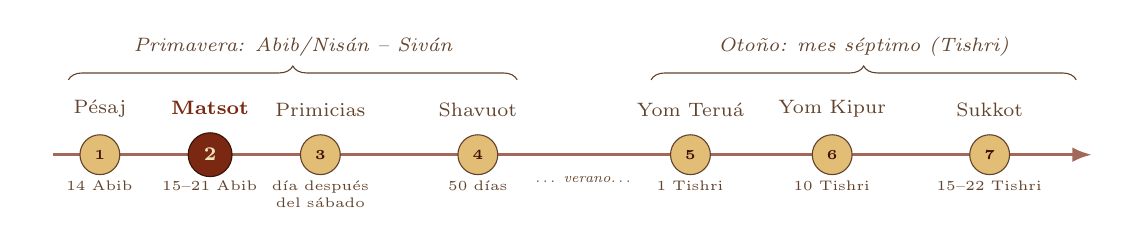
\begin{tikzpicture}[x=1cm,y=1cm,font=\scriptsize]
 \def\fiestaactual{2}
 \draw[line width=1.2pt,tierraroja!70,-{Latex[length=2.5mm]}] (0,0) -- (13.2,0);
 \draw[decorate,decoration={brace,amplitude=5pt},sepia] (0.2,0.95) -- (5.9,0.95) node[midway,above=5pt,font=\scriptsize\itshape]{Primavera: Abib/Nisán -- Siván};
 \draw[decorate,decoration={brace,amplitude=5pt},sepia] (7.6,0.95) -- (13.0,0.95) node[midway,above=5pt,font=\scriptsize\itshape]{Otoño: mes séptimo (Tishri)};
 \foreach \n/\x/\t/\d in {1/0.6/Pésaj/{14 Abib},2/2.0/Matsot/{15--21 Abib},3/3.4/Primicias/{día después del sábado},4/5.4/Shavuot/{50 días},5/8.1/Yom Teruá/{1 Tishri},6/9.9/Yom Kipur/{10 Tishri},7/11.9/Sukkot/{15--22 Tishri}}{
   \ifnum\n=\fiestaactual
     \node[circle,fill=tierraroja,draw=caferojizo,minimum size=5.5mm,text=papiro,font=\scriptsize\bfseries] at (\x,0) {\n};
     \node[above=3pt,font=\scriptsize\bfseries,text=tierraroja] at (\x,0.28) {\t};
   \else
     \node[circle,fill=mostaza!70,draw=sepia,minimum size=4.5mm,text=caferojizo,font=\tiny\bfseries] at (\x,0) {\n};
     \node[above=3pt,text=sepia] at (\x,0.25) {\t};
   \fi
   \node[below=6pt,text width=1.6cm,align=center,font=\tiny,text=sepia] at (\x,0) {\d};}
 \node[font=\tiny\itshape,text=sepia] at (6.75,-0.32) {\ldots\ verano\ldots};
\end{tikzpicture}}\par\nopagebreak
{\footnotesize\color{sepia}\textit{Figura 1.} El ciclo de Levítico 23: la fiesta de los Panes sin Levadura en su lugar. \textit{Nota.} Esquema estándar de la serie.}
\end{minipage}\end{center}

La fiesta ocupa el segundo lugar del ciclo y la semana entera que sigue a la Pascua. Dentro de esa semana cae el día de la gavilla de las primicias (Lv 23:9--14), que la serie estudia por separado, de modo que las tres fiestas de primavera forman una secuencia: la sangre que salva de la muerte, la salida que libra del cautiverio y la primicia que se presenta ante Dios.

%===================================================================
\section{El texto: la ley de los ázimos}

\subsection{El texto ancla: Levítico 23:6--8}
En el ``reglamento del culto'' de Levítico 23 la fiesta recibe tres versículos, con las fórmulas que se repiten a lo largo del capítulo: fecha, nombre, duración, convocación santa, prohibición de trabajo servil y ofrenda encendida.

\hebverso{וּבַחֲמִשָּׁה עָשָׂר יוֹם לַחֹדֶשׁ הַזֶּה חַג הַמַּצּוֹת לַיהוָה \\ שִׁבְעַת יָמִים מַצּוֹת תֹּאכֵלוּ}
\begin{cita}Y a los quince días de este mes es la fiesta solemne de los panes sin levadura a \SENOR; siete días comeréis panes sin levadura. El primer día tendréis santa convocación; ningún trabajo de siervos haréis. Y ofreceréis a \SENOR{} siete días ofrenda encendida; el séptimo día será santa convocación; ningún trabajo de siervo haréis.\fuente{(Lv 23:6--8)}\end{cita}

El nombre hebreo es \heb{חַג הַמַּצּוֹת} (\emph{jag hamatsot}), ``la fiesta de las \emph{matsot}''. \emph{Jag} es la fiesta de peregrinación, la que se celebra subiendo al santuario (la misma raíz que el árabe \emph{hajj}); \emph{matsot} es el plural de \emph{matsá}, la torta sin leudar. La RVR1960 traduce ``fiesta solemne de los panes sin levadura''; la RV1909 decía ``fiesta de los ázimos'', palabra que viene del griego \grc{ἄζυμα} a través del latín \emph{azyma}. El versículo 6 dice ``a \SENOR'' (\heb{לַיהוָה}): la fiesta pertenece al \SENOR, como todas las \emph{moadim} del capítulo (Lv 23:2, 4), y no a Israel ni a Moisés.

Los tres versículos tienen una disposición simétrica. Al centro va ``siete días'', dicho dos veces (vv.~6 y 8), siete de comer \emph{matsot} y siete de ofrenda encendida; en los bordes, el primer día y el séptimo, cada uno con la misma doble fórmula, \heb{מִקְרָא־קֹדֶשׁ} (\emph{mikrá kódesh}, ``santa convocación'') y \heb{כָּל־מְלֶאכֶת עֲבֹדָה לֹא תַעֲשׂוּ} (``ningún trabajo de siervos haréis''). La semana queda así encerrada entre dos días santos, como un texto entre paréntesis.

\subsection{Las leyes de la fiesta en el Pentateuco}
Levítico es solo una de las leyes de la fiesta. Éxodo da la institución en el marco del relato (12:14--20) y la repite como discurso de Moisés al pueblo (13:3--10); el Código de la Alianza y el Decálogo cultual la ponen a la cabeza de las tres fiestas de peregrinación (23:15; 34:18); Números fija los sacrificios diarios (28:17--25); Deuteronomio la une a la Pascua en el santuario central y le da la explicación más honda, la del ``pan de aflicción'' (16:3). La tabla siguiente reúne lo que cada texto aporta.

\begin{center}\begin{minipage}{\linewidth}\centering\small\renewcommand{\arraystretch}{1.2}
\begin{tabular}{@{}L{2.4cm}L{3.6cm}L{9.6cm}@{}}
\toprule
\textbf{Texto} & \textbf{Fecha y duración} & \textbf{Qué añade} \\ \midrule
Éx 12:14--20 & 14 por la tarde al 21 por la tarde (v.~18); siete días & ``Memoria'' y ``estatuto perpetuo''; quitar la \emph{se'or} de las casas ``el primer día''; pena de \emph{karet} para quien coma \emph{jamets}; 1.º y 7.º día \emph{mikrá kódesh}; solo se permite preparar comida; vale ``así extranjero como natural''. Motivo: ``en este mismo día saqué vuestras huestes'' (v.~17). \\
Éx 12:33--39 & la mañana de la salida & El origen narrado: masa ``antes que se leudase'', las artesas sobre los hombros, tortas sin levadura ``pues no había leudado'' (vv.~34, 39). \\
Éx 13:3--10 & ``en el mes de Abib'' & Discurso de Moisés: ``Tened memoria de este día''; el 7.º día es \emph{jag}; ni leudado ni levadura ``en todo tu territorio''; la instrucción al hijo (v.~8); señal en la mano y memoria entre los ojos (v.~9). \\
Éx 23:15 & ``en el mes de Abib'' & Primera de las tres fiestas de peregrinación; nadie se presentará ante Dios con las manos vacías. \\
Éx 34:18 & ``en el mes de Abib'' & Repite 23:15 en la renovación del pacto, tras el becerro de oro. \\
Lv 23:6--8 & 15 al 21 del primer mes & La fiesta dentro del calendario completo; ofrenda encendida los siete días; ``trabajo de siervos'' prohibido en los días santos. \\
Nm 28:17--25 & 15 al 21; siete días & Los sacrificios de cada día: dos becerros, un carnero, siete corderos, ofrenda de harina y un macho cabrío ``por expiación'', además del holocausto continuo. \\
Dt 16:3--4, 8 & ``seis días'' más el séptimo como \emph{atséret} & Unión con la Pascua ``en el lugar que \SENOR{} escogiere''; ``pan de aflicción, porque aprisa saliste''; recordar ``todos los días de tu vida''; el 7.º día es \emph{atséret}. \\
\bottomrule
\end{tabular}\par\nopagebreak
{\footnotesize\color{sepia}\textit{Tabla 1.} Tabla sinóptica de las leyes de los Panes sin Levadura. \textit{Nota.} Elaboración propia con la BHS y la RVR1960.}
\end{minipage}\end{center}

\subsection{Éxodo 12: la ley dentro de la noche}
El texto más extenso está en Éxodo 12, y vale la pena fijarse en dónde está: la ley de una fiesta anual aparece antes de que ocurra el hecho que conmemora. Dios ordena recordar una salida que todavía no ha sucedido.

\hebverso{וּשְׁמַרְתֶּם אֶת־הַמַּצּוֹת כִּי בְּעֶצֶם הַיּוֹם הַזֶּה הוֹצֵאתִי אֶת־צִבְאוֹתֵיכֶם מֵאֶרֶץ מִצְרָיִם}
\begin{cita}Este día os será en memoria, y lo celebraréis como fiesta solemne para \SENOR{} durante vuestras generaciones; por estatuto perpetuo lo celebraréis. Siete días comeréis panes sin levadura; y así el primer día haréis que no haya levadura en vuestras casas; porque cualquiera que comiere leudado desde el primer día hasta el séptimo, será cortado de Israel.\fuente{(Éx 12:14--15)}\end{cita}
\begin{cita}Y guardaréis la fiesta de los panes sin levadura, porque en este mismo día saqué vuestras huestes de la tierra de Egipto; por tanto, guardaréis este mandamiento en vuestras generaciones por costumbre perpetua.\fuente{(Éx 12:17)}\end{cita}

Tres frases del pasaje sostienen lo que sigue. ``Este día os será en memoria'' (\heb{לְזִכָּרוֹן}, \emph{lezikarón}) hace de la fiesta un memorial, una forma de recordar con el cuerpo. ``Por estatuto perpetuo'' (\heb{חֻקַּת עוֹלָם}, \emph{jukat olam}) extiende su vigencia ``durante vuestras generaciones''. Y ``en este mismo día'' (\heb{בְּעֶצֶם הַיּוֹם הַזֶּה}, \emph{be'étsem hayom hazé}, literalmente ``en el hueso de este día'') fija la fecha en la del hecho, sin aproximación. La expresión aparece tres veces en el capítulo (vv.~17, 41, 51) y vuelve en Jos 5:11, cuando Israel come por primera vez los ázimos del fruto de Canaán. En toda la Biblia hebrea son catorce casos, y siempre marcan fechas fundacionales: la entrada en el arca (Gn 7:13), la circuncisión de Abraham (Gn 17:23, 26), los días santos de Lv 23 (vv.~21, 28--30), la muerte anunciada de Moisés (Dt 32:48) y las fechas de Ezequiel (Ez 24:2; 40:1) (conteo propio sobre el Códice de Leningrado).

\subsection{Deuteronomio 16: pan de aflicción}
Deuteronomio, que habla a la generación que va a entrar en la tierra, explica el pan:

\hebverso{שִׁבְעַת יָמִים תֹּאכַל־עָלָיו מַצּוֹת לֶחֶם עֹנִי כִּי בְחִפָּזוֹן יָצָאתָ מֵאֶרֶץ מִצְרַיִם}
\begin{cita}No comerás con ella pan con levadura; siete días comerás con ella pan sin levadura, pan de aflicción, porque aprisa saliste de tierra de Egipto; para que todos los días de tu vida te acuerdes del día en que saliste de la tierra de Egipto.\fuente{(Dt 16:3)}\end{cita}

El versículo explica el pan dos veces. Es \heb{לֶחֶם עֹנִי} (\emph{lejem oni}), ``pan de aflicción'', el pan de la servidumbre y de la pobreza; y es pan de la prisa, \heb{כִּי בְחִפָּזוֹן יָצָאתָ}, ``porque aprisa saliste''. La palabra \emph{jipazón} (``prisa, huida apresurada'') aparece solo tres veces en la Biblia hebrea: en la noche de la Pascua (``lo comeréis apresuradamente'', Éx 12:11), aquí y en Is 52:12, donde el profeta anuncia un éxodo nuevo invirtiendo la imagen: ``no saldréis apresurados, ni iréis huyendo; porque \SENOR{} irá delante de vosotros'' (conteo propio del lema sobre el Códice de Leningrado). Un mismo pan recuerda, entonces, la aflicción de la que se salió y la urgencia con que se salió.

\begin{nota}[Precisión]
Dt 16:8 dice ``seis días comerás pan sin levadura, y el séptimo día será fiesta solemne'' (\emph{atséret}), mientras Éx 12:15 y Lv 23:6 dicen ``siete días''. La tensión se discute en la sección~\ref{sec:textual}. Baste aquí con señalar que Deuteronomio no elimina el séptimo día; lo nombra con otra palabra.
\end{nota}

%===================================================================
\section{Lectura histórica}

\subsection{Abib: el mes de la espiga}
La fiesta cae ``en el mes de Abib'' (Éx 13:4; 23:15; 34:18; Dt 16:1). \heb{אָבִיב} (\emph{aviv}) designa la espiga ya formada pero todavía verde; en la séptima plaga ``la cebada estaba ya espigada'' (\emph{aviv}, Éx 9:31). En la tierra de Israel, ese momento coincide con el fin de las lluvias de invierno y el comienzo de la siega de la cebada, que se abre con la gavilla de las primicias dentro de la misma semana (Lv 23:10--11). Después del exilio el mes se llamó Nisán, con nombre babilonio (Neh 2:1; Est 3:7). Abib/Nisán es el primer mes, ``principio de los meses'' (Éx 12:2).

La coincidencia agrícola es real y explica que la fiesta sea de primavera. La razón que el texto da, sin embargo, es la salida y no la cosecha: ``porque en el mes de Abib saliste de Egipto'' (Éx 34:18). Israel celebra un hecho de su historia dentro del ciclo de las estaciones, y es el hecho lo que se recuerda.

\subsection{La prisa de la salida}
El relato de Éxodo 12 explica el pan sin levadura con una escena de cocina:

\hebverso{וַיִּשָּׂא הָעָם אֶת־בְּצֵקוֹ טֶרֶם יֶחְמָץ מִשְׁאֲרֹתָם צְרֻרֹת בְּשִׂמְלֹתָם עַל־שִׁכְמָם}
\begin{cita}Y los egipcios apremiaban al pueblo, dándose prisa a echarlos de la tierra; porque decían: Todos somos muertos. Y llevó el pueblo su masa antes que se leudase, sus masas envueltas en sus sábanas sobre sus hombros.\fuente{(Éx 12:33--34)}\end{cita}

El hebreo dice que el pueblo cargó su \heb{בָּצֵק} (\emph{batsek}, ``masa'') ``antes de que leudara'' (\heb{טֶרֶם יֶחְמָץ}), y sus \heb{מִשְׁאֲרֹתָם} (\emph{mish'arotam}), ``sus artesas'', envueltas en los mantos. La RVR1960 traduce ``sus masas'', pero \emph{mish'éret} es la artesa de amasar, la misma palabra de la segunda plaga, cuando las ranas entraron ``en tus hornos y en tus artesas'' (Éx 8:3 [7:28]). Los israelitas salieron, pues, con la artesa al hombro y la masa dentro. Unos versículos después el narrador cierra la escena:

\begin{cita}Y cocieron tortas sin levadura de la masa que habían sacado de Egipto, pues no había leudado, porque al echarlos fuera los egipcios, no habían tenido tiempo ni para prepararse comida.\fuente{(Éx 12:39)}\end{cita}

El verbo es fuerte, \heb{כִּי־גֹרְשׁוּ מִמִּצְרַיִם} (\emph{ki gorshú}), ``porque fueron expulsados'', y Dios lo había anunciado con la misma raíz \emph{garash}: ``os echará de aquí del todo'' (Éx 11:1). Hay en ello una ironía que la fiesta conserva: el faraón que no quería dejar ir al pueblo termina expulsándolo con tanta urgencia que no queda tiempo para el pan.

\subsection{Pan de pastores, pan de pobres}
La \emph{matsá} no fue inventada para la fiesta. Era el pan rápido de una cocina sin horno fijo, harina, agua y fuego, y la Biblia lo muestra en escenas de hospitalidad apurada. Abraham pide a Sara tortas (\heb{עֻגוֹת}, \emph{ugot}) para los visitantes, ``de prisa'' (Gn 18:6); Lot cuece \emph{matsot} para los ángeles (Gn 19:3); Gedeón prepara un cabrito y \emph{matsot} para el ángel (Jue 6:19); la mujer de Endor mata un ternero, ``y tomó harina y la amasó, y coció de ella panes sin levadura'' para Saúl (1~S 28:24). Los estudios sobre la vida cotidiana en Oriente describen todavía el pan de pastores y beduinos, cocido sobre brasas o piedras calientes, sin fermentar (Wight, 1953). El pan leudado, en cambio, pide tiempo, una porción de masa madre guardada del día anterior y una casa estable.

Por eso la \emph{matsá} reúne las dos explicaciones de Deuteronomio: es pan de pobres y de servidumbre (``pan de aflicción'') y pan de caminantes (``porque aprisa saliste''). Comerlo siete días es ponerse, por una semana, en la condición de los que salieron, sin casa propia, sin tiempo, con lo que se puede cargar al hombro.

\begin{nota}[Precisión: el origen de la fiesta según la crítica histórica]
Desde el siglo~\textsc{xix} muchos historiadores de la religión sostienen que Pésaj y Matsot fueron al principio dos fiestas distintas: una de pastores (el cordero de primavera) y otra de agricultores (el comienzo de la siega de la cebada, con pan de grano nuevo sin la levadura vieja), unidas después en la historia de Israel y fundidas en Deuteronomio 16 (de Vaux, 1985; véase la discusión en Propp, 1999). Es una hipótesis académica, no un dato del texto. El Pentateuco presenta las dos fiestas unidas desde su institución (Éx 12) y da a los ázimos un origen histórico, la masa sin leudar de la salida (Éx 12:34, 39), antes que agrícola. Sigo aquí el texto y dejo constancia de la hipótesis por honestidad.
\end{nota}

\subsection{El itinerario de la salida}
El texto da con precisión el punto de partida y la fecha: ``De Ramesés salieron en el mes primero, a los quince días del mes primero; el segundo día de la pascua salieron los hijos de Israel con mano poderosa, a vista de todos los egipcios'' (Nm 33:3). La expresión hebrea es \heb{מִמָּחֳרַת הַפֶּסַח} (\emph{mimojorat hapésaj}), ``al día siguiente de la Pascua''; aparece solo aquí y en Jos 5:11, cuando Israel, ya en Canaán, ``al otro día de la pascua'' come los panes sin levadura del fruto de la tierra (conteo propio), de modo que la salida y la entrada quedan unidas por la misma frase y por el mismo pan.

Las etapas se leen en dos textos paralelos, el relato (Éx 12:37; 13:20; 14:2) y la lista de estaciones (Nm 33:5--8).

\begin{cita}Partieron, pues, los hijos de Israel de Ramesés, y acamparon en Sucot. Salieron de Sucot y acamparon en Etam, que está al confín del desierto. Salieron de Etam y volvieron sobre Pi-hahirot, que está delante de Baal-zefón, y acamparon delante de Migdol.\fuente{(Nm 33:5--7, trad. propia)}\end{cita}

\begin{cita}Di a los hijos de Israel que den la vuelta y acampen delante de Pi-hahirot, entre Migdol y el mar hacia Baal-zefón; delante de él acamparéis junto al mar.\fuente{(Éx 14:2)}\end{cita}

Dios evita ``el camino de la tierra de los filisteos, que estaba cerca'' (Éx 13:17), la ruta militar de la costa, y lleva al pueblo ``por el camino del desierto del Mar Rojo'' (13:18). Desde Etam, ``a la entrada del desierto'' (13:20), ordena volver (14:2), y el pueblo acampa encerrado entre el desierto y el mar, para que el faraón piense que ``encerrados están en la tierra'' (14:3). Allí lo alcanzan los carros egipcios (14:9), y esa noche el mar se retira ``por recio viento oriental toda aquella noche'' (14:21).

La identificación de los lugares sigue discutida. Ramsés suele identificarse con Pi-Ramsés, en Qantir y Tell el-Dab`a, en el delta oriental; Sucot, con la región de Tjeku en el Wadi Tumilat (quizá Tell el-Maskhuta); Etam, Pi-hahirot, Migdol y Baal-zefón no tienen identificación segura, y el \heb{יַם־סוּף} (\emph{Yam Suf}, ``mar de juncos'', que la LXX tradujo ``Mar Rojo'') se ha buscado en los lagos del istmo de Suez (Ballah, Timsah, Amargos), en el golfo de Suez o en la laguna Sirbónica de la costa (Hoffmeier, 1997; Kitchen, 2003). El mapa siguiente es esquemático y muestra las regiones y las dos rutas más propuestas, sin pretender un trazado demostrado.

\begin{center}\begin{minipage}{\linewidth}\centering
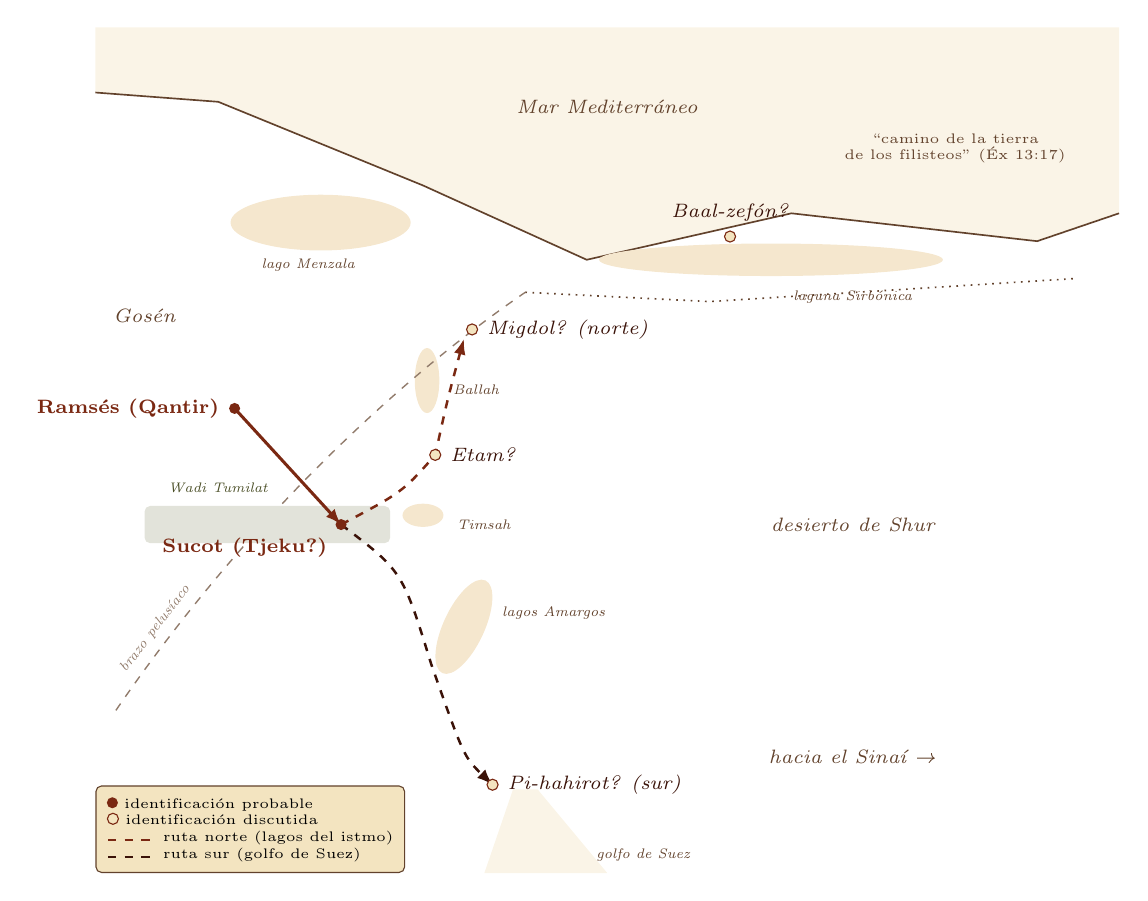
\begin{tikzpicture}[x=5.2cm,y=5.9cm,font=\scriptsize]
 \fill[mostaza!12] (31.5,31.62) -- (31.5,31.48) -- (31.8,31.46) -- (32.3,31.28) -- (32.7,31.12) -- (33.2,31.22) -- (33.8,31.16) -- (34.0,31.22) -- (34.0,31.62) -- cycle;
 \draw[sepia,line width=0.6pt] (31.5,31.48) -- (31.8,31.46) -- (32.3,31.28) -- (32.7,31.12) -- (33.2,31.22) -- (33.8,31.16) -- (34.0,31.22);
 \node[font=\scriptsize\itshape,text=sepia] at (32.75,31.45) {Mar Mediterráneo};
 \fill[mostaza!25] (32.05,31.20) ellipse (0.22 and 0.06);
 \node[font=\tiny\itshape,text=sepia] at (32.02,31.11) {lago Menzala};
 \fill[mostaza!25] (33.15,31.12) ellipse (0.42 and 0.035);
 \node[font=\tiny\itshape,text=sepia,align=center] at (33.35,31.04) {laguna Sirbónica};
 \fill[mostaza!25] (32.31,30.86) ellipse (0.03 and 0.07);
 \node[font=\tiny\itshape,text=sepia,anchor=west] at (32.35,30.84) {Ballah};
 \fill[mostaza!25] (32.30,30.57) ellipse (0.05 and 0.025);
 \node[font=\tiny\itshape,text=sepia,anchor=west] at (32.36,30.55) {Timsah};
 \fill[mostaza!25,rotate around={-25:(32.40,30.33)}] (32.40,30.33) ellipse (0.05 and 0.11);
 \node[font=\tiny\itshape,text=sepia,anchor=west] at (32.47,30.36) {lagos Amargos};
 \fill[mostaza!12] (32.52,29.98) -- (32.58,29.98) -- (32.75,29.80) -- (32.45,29.80) -- cycle;
 \node[font=\tiny\itshape,text=sepia,anchor=west] at (32.70,29.84) {golfo de Suez};
 \draw[sepia!70,line width=0.5pt,dashed] (31.55,30.15) .. controls (31.9,30.6) and (32.3,30.9) .. (32.55,31.05) node[pos=0.12,sloped,above,font=\tiny\itshape]{brazo pelusíaco};
 \fill[oliva!18,rounded corners=2pt] (31.62,30.51) rectangle (32.22,30.59);
 \node[font=\tiny\itshape,text=oliva!80!black] at (31.80,30.63) {Wadi Tumilat};
 \node[font=\scriptsize\itshape,text=sepia] at (31.62,31.0) {Gosén};
 \node[font=\scriptsize\itshape,text=sepia] at (33.35,30.55) {desierto de Shur};
 \node[font=\scriptsize\itshape,text=sepia] at (33.35,30.05) {hacia el Sinaí \textrightarrow};
 \draw[sepia,line width=0.6pt,dotted] (32.55,31.05) -- (33.0,31.03) -- (33.9,31.08);
 \node[font=\tiny,text=sepia,align=center] at (33.6,31.36) {``camino de la tierra\\ de los filisteos'' (Éx 13:17)};
 \draw[tierraroja,line width=1.1pt,-{Latex[length=2mm]}] (31.84,30.80) -- (32.10,30.55);
 \draw[tierraroja,line width=0.9pt,dashed,-{Latex[length=2mm]}] (32.10,30.55) .. controls (32.25,30.62) .. (32.33,30.70) .. controls (32.36,30.82) .. (32.40,30.95);
 \draw[caferojizo,line width=0.9pt,dashed,-{Latex[length=2mm]}] (32.10,30.55) .. controls (32.25,30.45) .. (32.32,30.25) .. controls (32.40,30.05) .. (32.47,29.99);
 \foreach \x/\y/\n/\p in {31.84/30.80/{Ramsés (Qantir)}/left, 32.10/30.55/{Sucot (Tjeku?)}/below left}{
   \fill[tierraroja] (\x,\y) circle (2pt); \node[\p=2pt,font=\scriptsize\bfseries,text=tierraroja] at (\x,\y) {\n};}
 \foreach \x/\y/\n/\p in {32.33/30.70/{Etam?}/right, 32.42/30.97/{Migdol? (norte)}/right, 32.47/29.99/{Pi-hahirot? (sur)}/right, 33.05/31.17/{Baal-zefón?}/above}{
   \draw[tierraroja,fill=papiro] (\x,\y) circle (2pt); \node[\p=2pt,font=\scriptsize\itshape,text=caferojizo] at (\x,\y) {\n};}
 \node[draw=sepia,fill=papiro,rounded corners=2pt,anchor=south west,align=left,font=\tiny,inner sep=4pt] at (31.5,29.8) {%
   \tikz[x=1cm,y=1cm]\fill[tierraroja] (0,0) circle (2pt); identificación probable\\
   \tikz[x=1cm,y=1cm]\draw[tierraroja,fill=papiro] (0,0) circle (2pt); identificación discutida\\
   \tikz[x=1cm,y=1cm]\draw[tierraroja,dashed,line width=0.9pt] (0,0)--(0.6,0); ruta norte (lagos del istmo)\\
   \tikz[x=1cm,y=1cm]\draw[caferojizo,dashed,line width=0.9pt] (0,0)--(0.6,0); ruta sur (golfo de Suez)};
\end{tikzpicture}\par\nopagebreak
{\footnotesize\color{sepia}\textit{Figura 2.} Mapa esquemático del itinerario de la salida (Éx 12:37; 13:17--20; 14:2; Nm 33:3--8). \textit{Nota.} Elaboración propia con coordenadas aproximadas; los lugares con signo de interrogación tienen identificación discutida (Hoffmeier, 1997; Kitchen, 2003).}
\end{minipage}\end{center}

\subsection{¿Cuándo cruzaron el mar? Tres cronologías}
El documento de referencia de la serie reconstruye los primeros días uno por uno. El 15 de Abib los israelitas salen de Gosén y Ramsés y se reúnen en Sucot; el 16 marchan a Etam; el 17 dan la vuelta por Pi-hahirot y acampan ante Migdol, donde el faraón los alcanza ``al tercer día de su partida'', y ese mismo día cruzan el mar; el 18 de Abib Israel se presenta ``por primera vez, definitivamente libre del faraón de Egipto'' ante Dios, como ``primicia de las naciones'' (Éx 19:5--6). El cómputo se apoya en Nm 33:1--7 y en Éx 14:9, y se enlaza con la gavilla de las primicias.

La tradición rabínica cuenta los días de otro modo. Rashi, comentando Éx 14:5 (``Y fue dado aviso al rey de Egipto que el pueblo huía''), explica que el faraón había enviado oficiales con Israel; cumplidos los tres días de camino que Moisés había pedido (Éx 3:18; 5:3), al ver que no volvían, avisaron al rey el cuarto día; el quinto y el sexto los persiguieron, y en la noche del séptimo bajaron al mar; a la mañana cantaron el Cántico, ``y ese fue el séptimo día de Pésaj; por eso leemos el Cántico el séptimo día''. La misma cronología aparece en el Seder Olam y en la Mekhiltá. Según ella, el cruce ocurrió el 21 de Nisán, el último día santo de la fiesta.

El texto bíblico es más sobrio que ambas reconstrucciones. Da una sola fecha, el 15 del primer mes (Nm 33:3); nombra las estaciones sin decir que cada una corresponda a un día de marcha; sitúa el cruce de noche (Éx 14:20--21) y el retorno del mar a su fuerza ``cuando amanecía'' (14:27). Después del mar, Israel anda ``tres días por el desierto'' hasta Mara (Éx 15:22; Nm 33:8).

\begin{center}\begin{minipage}{\linewidth}\centering\small\renewcommand{\arraystretch}{1.2}
\begin{tabular}{@{}L{1.5cm}L{4.5cm}L{4.6cm}L{4.9cm}@{}}
\toprule
\textbf{Abib} & \textbf{Lectura de la serie} & \textbf{Lo que el texto dice} & \textbf{Tradición rabínica} \\ \midrule
14 (tarde) & Pascua; muerte de los primogénitos & Pascua; la plaga ``a la medianoche'' (Éx 12:29) & Igual \\
15 & Salida de Gosén y Ramsés; campamento en Sucot & Única fecha explícita: salida de Ramsés ``al día siguiente de la Pascua'', ``con mano poderosa'' (Nm 33:3); campamento en Sucot (12:37) & Salida; primer día santo \\
16 & Marcha a Etam & Sucot $\rightarrow$ Etam ``a la entrada del desierto'' (13:20); sin fecha & Marcha \\
17 & Vuelta por Pi-hahirot; el faraón los alcanza ante Migdol ``al tercer día''; cruce del mar & Vuelta a Pi-hahirot (14:2); el faraón los alcanza ``junto al mar'' (14:9); sin fecha & Tercer día: fin del plazo pedido (Éx 3:18) \\
18 & Israel ``libre del faraón'', primicia de las naciones & --- & Los oficiales avisan al faraón (Rashi a Éx 14:5) \\
19--20 & --- & --- & Persecución \\
21 & Séptimo día santo & Séptimo día: \emph{mikrá kódesh} (Lv 23:8) & Cruce en la noche; Cántico del Mar en la mañana \\
\bottomrule
\end{tabular}\par\nopagebreak
{\footnotesize\color{sepia}\textit{Tabla 2.} Tres cronologías de la salida. \textit{Nota.} Elaboración propia con el documento de referencia de la serie, la RVR1960 y Rashi a Éx 14:5 (Sefaria).}
\end{minipage}\end{center}

\begin{nota}[Precisión]
Las dos cronologías completas son reconstrucciones. La de la serie lee cada estación de Nm 33:5--7 como un día de marcha y toma el ``tercer día'' de la persecución; la rabínica parte de los ``tres días de camino'' pedidos al faraón y del uso litúrgico del Cántico el séptimo día. Josefo, que resume el viaje, hace llegar a los hebreos a Beelsefón ``al tercer día'' (\emph{Antigüedades} 2.315 [2.15.1]: \emph{on the third day they came to a place called Beelzephon}, en la traducción de Whiston), un dato antiguo cercano a la lectura de la serie. Éx 14:9 dice que el faraón los alcanzó acampados junto al mar, pero no dice ``al tercer día''; esa precisión es un cálculo y no una cita. Ninguna de las dos reconstrucciones contradice el texto, y ninguna está explícita en él.
\end{nota}

\begin{center}\begin{minipage}{\linewidth}\centering
\begin{tikzpicture}[x=1.95cm,y=1cm,font=\scriptsize]
 \node[draw=sepia,fill=mostaza!25,minimum width=1.6cm,minimum height=1.1cm,align=center,rounded corners=2pt] at (0,0) {\textbf{14}\\[-1pt]Pésaj\\[-1pt]{\tiny (tarde)}};
 \foreach \i/\d in {1/15,2/16,3/17,4/18,5/19,6/20,7/21}{
   \ifnum\i=1 \def\col{tierraroja}\def\tx{papiro}\else\ifnum\i=7 \def\col{tierraroja}\def\tx{papiro}\else\def\col{mostaza!20}\def\tx{caferojizo}\fi\fi
   \node[draw=caferojizo,fill=\col,text=\tx,minimum width=1.6cm,minimum height=1.1cm,align=center,rounded corners=2pt] (d\i) at (\i,0) {\textbf{\d}\\[-1pt]{\tiny día \i}};}
 \node[below=1pt,font=\tiny\bfseries,text=tierraroja] at (d1.south) {\emph{mikrá kódesh}};
 \node[below=1pt,font=\tiny\bfseries,text=tierraroja] at (d7.south) {\emph{mikrá kódesh}};
 \draw[decorate,decoration={brace,amplitude=5pt,mirror},sepia] (1.6,-0.95) -- (6.4,-0.95) node[midway,below=5pt,font=\tiny\itshape]{días intermedios: se comen \emph{matsot}; el trabajo está permitido};
 \node[font=\tiny\bfseries,text=tierraroja,anchor=east] at (-0.45,1.55) {Serie};
 \foreach \i/\t in {1/{Ramsés $\rightarrow$ Sucot},2/{Sucot $\rightarrow$ Etam},3/{Migdol: cruce},4/{``libres del faraón''}}{
   \node[text width=1.7cm,align=center,font=\tiny,text=caferojizo] at (\i,1.55) {\t};
   \draw[mostaza!80!tierraroja,-{Latex[length=1.5mm]}] (\i,1.25) -- (\i,0.6);}
 \node[font=\tiny\bfseries,text=sepia,anchor=east] at (-0.45,-2.1) {Tradición};
 \foreach \i/\t in {1/{salida},4/{aviso al faraón},5/{persecución},6/{persecución},7/{cruce y Cántico (Éx 15)}}{
   \node[text width=1.7cm,align=center,font=\tiny\itshape,text=sepia] at (\i,-2.1) {\t};}
 \node[font=\tiny\bfseries,text=oliva!80!black,anchor=east] at (-0.45,2.35) {Texto};
 \node[text width=3.4cm,align=center,font=\tiny,text=oliva!80!black] at (1,2.35) {única fecha: salida el 15 (Nm 33:3)};
 \node[text width=3.6cm,align=center,font=\tiny,text=oliva!80!black] at (6.2,2.35) {Lv 23:8: el 7.º día, convocación santa};
\end{tikzpicture}\par\nopagebreak
{\footnotesize\color{sepia}\textit{Figura 3.} La semana de los Panes sin Levadura con los días santos y los hechos de la salida según la serie, el texto y la tradición rabínica. \textit{Nota.} Elaboración propia.}
\end{minipage}\end{center}

La cronología rabínica tiene un fruto litúrgico que vale la pena recoger: en la sinagoga, el séptimo día de la fiesta se lee el Cántico del Mar, y el Talmud fija para ese día la lectura de ``Y luego que Faraón dejó ir al pueblo'' (Éx 13:17--15:26; Meguilá 31a). La semana que empieza con la salida de Ramsés termina así con el canto de los libres: ``Cantaré yo a \SENOR, porque se ha magnificado grandemente; ha echado en el mar al caballo y al jinete'' (Éx 15:1). Haya ocurrido el cruce el día 17 o el 21, la semana de la fiesta abarca la liberación completa, la salida y el mar.

\begin{nota}[Precisión: la fecha del éxodo]
La serie fecha la salida en el año 1529/1530 a.\,e.\,c., según su propio cómputo. La cronología interna de la Biblia, que cuenta 480 años desde la salida hasta el cuarto año de Salomón (1~R 6:1; ca. 966 a.\,e.\,c.), da una fecha ``temprana'' cercana a 1446 a.\,e.\,c. Muchos historiadores prefieren una fecha ``tardía'', hacia 1260 a.\,e.\,c., bajo Ramsés~II, por el nombre de la ciudad de Ramsés (Éx 1:11) y por la arqueología de Canaán (Kitchen, 2003; Hoffmeier, 1997). La diferencia afecta a la cronología absoluta y no al calendario de la fiesta; el 15 de Abib es el mismo en cualquier hipótesis. Los 430 años de Éx 12:40--41 se cuentan en Egipto según el texto masorético; la LXX y el Pentateuco Samaritano añaden ``y en la tierra de Canaán'', y Pablo cuenta 430 años desde la promesa a Abraham hasta la ley (Gá 3:17).
\end{nota}

\subsection{La fiesta en la historia de Israel}
Después del desierto, la fiesta reaparece en momentos de comienzo o de restauración.

\paragraph{Gilgal (Jos 5:10--12).} La primera Pascua en Canaán se celebra en los llanos de Jericó, tras la circuncisión de la nueva generación. ``Al otro día de la pascua comieron del fruto de la tierra, los panes sin levadura, y en el mismo día espigas nuevas tostadas'' (Jos 5:11), y al día siguiente cesó el maná: los primeros ázimos de grano de Canaán marcan el paso del pan del cielo al pan de la tierra.

\paragraph{Salomón (2~Cr 8:13).} El templo ofrece holocaustos ``en las fiestas solemnes, tres veces en el año, esto es, en la fiesta de los panes sin levadura, en la fiesta de las semanas, y en la fiesta de los tabernáculos''. Los Ázimos encabezan las tres fiestas de peregrinación, como en Éx 23:15 y Dt 16:16.

\paragraph{Ezequías (2~Cr 30).} El rey reforma el culto y convoca a todo Israel, incluido el norte, a celebrar ``la fiesta solemne de los panes sin levadura en el mes segundo'' (30:13), aplicando la provisión de Nm 9:10--11 para los impuros y los que estaban lejos. La fiesta se celebra ``por siete días con grande gozo'' (30:21), y la asamblea decide celebrar ``otros siete días'' (30:23), la única fiesta de los Ázimos duplicada que narra la Biblia.

\paragraph{Josías (2~R 23:21--23; 2~Cr 35:17).} Tras el hallazgo del libro de la ley, Josías celebra una Pascua como no se había hecho ``desde los tiempos de los jueces''; Crónicas añade que celebraron la Pascua ``y la fiesta solemne de los panes sin levadura por siete días''.

\paragraph{Ezequiel (45:21--24).} En la visión del templo restaurado, el príncipe ofrece cada uno de los siete días de la fiesta siete becerros y siete carneros. La sección textual vuelve sobre la forma de 45:21.

\paragraph{Esdras (6:19--22).} Los que volvieron del exilio, ya terminado el segundo templo (515 a.\,e.\,c.), celebran la Pascua y ``con regocijo la fiesta solemne de los panes sin levadura siete días, por cuanto \SENOR{} los había alegrado'' (Esd 6:22). Con ellos comen todos los que se habían apartado de las inmundicias de las gentes de la tierra (6:21), y la fiesta de la salida de Egipto resulta ser también la de una comunidad separada del mundo que la rodea.

\subsection{El Segundo Templo}
En el período del Segundo Templo la fiesta está bien documentada, siempre unida a la Pascua.

\paragraph{Elefantina (419 a.\,e.\,c.).} En la colonia militar judía del Alto Egipto se encontró una carta, conocida como el papiro de la Pascua (Cowley~21), en la que un tal Jananías transmite la orden de observar la fiesta entre el 15 y el 21 de Nisán: guardarse puros, no beber bebidas fermentadas, no comer nada leudado y guardar lo leudado fuera de la vista. El texto está dañado y en parte reconstruido (Porten, 1968), pero basta para mostrar la fiesta observada en la diáspora siglos antes del Nuevo Testamento.

\paragraph{Qumrán.} El Rollo del Templo (11QT 17:10--16) prescribe, después de la Pascua del 14, la fiesta de los panes sin levadura del 15 al 21, con convocación santa el primer día y holocaustos diarios (Yadin, 1983).

\paragraph{Filón y Josefo.} Filón de Alejandría dedica a la fiesta un pasaje de \emph{De specialibus legibus} (2.150--161) y lee el pan sin levadura como alimento en su estado natural y memoria de la migración. Josefo la describe con exactitud: al día quince ``sucede a la Pascua la fiesta de los panes ázimos, que dura siete días'' (\emph{Antigüedades} 3.249, trad. propia), aunque en otros pasajes usa los nombres como equivalentes: ``la fiesta de los panes ázimos, que llamamos Pascua'' (\emph{Antigüedades} 14.21, trad. propia). En otro lugar habla de una fiesta ``de ocho días'' llamada de los ázimos (\emph{Antigüedades} 2.317), contando el 14 con los siete siguientes.

\paragraph{El Nuevo Testamento.} Los evangelios conocen la misma fusión: ``Dos días después era la pascua, y la fiesta de los panes sin levadura'' (Mc 14:1); ``Estaba cerca la fiesta de los panes sin levadura, que se llama la pascua'' (Lc 22:1). Lucas fecha con la fiesta dos episodios de Hechos: el arresto de Pedro (``eran entonces los días de los panes sin levadura'', Hch 12:3) y un viaje de Pablo (``pasados los días de los panes sin levadura, navegamos de Filipos'', Hch 20:6).

\paragraph{La Misná (ca. 200 e.\,c.).} El tratado \emph{Pesajim} (caps. 1--3) codifica la búsqueda del \emph{jamets} la noche del 14 ``a la luz de una lámpara'' (\emph{bedikat jamets}, 1:1), la hora límite para comerlo y su quema (\emph{biur}, 1:4; 2:1), y los cinco cereales con que se cumple la obligación de la \emph{matsá} (2:5). Es una fuente posterior que sistematiza prácticas del Segundo Templo, y se estudia en la sección~\ref{sec:tradicion}.

\begin{center}\begin{minipage}{\linewidth}\centering
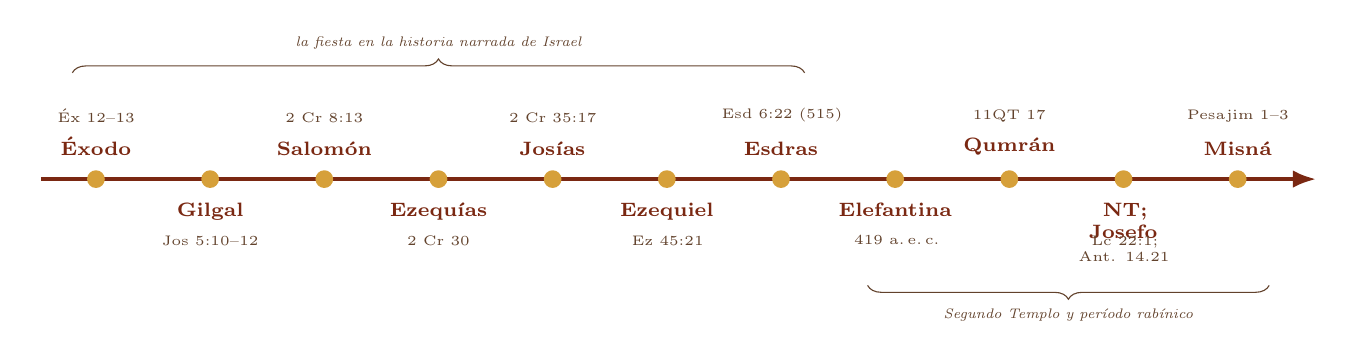
\begin{tikzpicture}[x=1cm,y=1cm,font=\scriptsize]
 \draw[line width=1.6pt,tierraroja,-{Latex[length=3mm]}] (-0.3,0) -- (15.9,0);
 \foreach \x/\a/\b/\s in {0.4/{Éxodo}/{Éx 12--13}/1, 1.85/{Gilgal}/{Jos 5:10--12}/-1, 3.3/{Salomón}/{2 Cr 8:13}/1, 4.75/{Ezequías}/{2 Cr 30}/-1, 6.2/{Josías}/{2 Cr 35:17}/1, 7.65/{Ezequiel}/{Ez 45:21}/-1, 9.1/{Esdras}/{Esd 6:22 (515)}/1, 10.55/{Elefantina}/{419 a.\,e.\,c.}/-1, 12.0/{Qumrán}/{11QT 17}/1, 13.45/{NT; Josefo}/{Lc 22:1; Ant. 14.21}/-1, 14.9/{Misná}/{Pesajim 1--3}/1}{
   \fill[mostaza] (\x,0) circle (3.2pt);
   \ifnum\s=1
     \node[above=5pt,font=\scriptsize\bfseries,text=tierraroja,text width=1.5cm,align=center] at (\x,0) {\a};
     \node[above=17pt,font=\tiny,text=sepia,text width=1.5cm,align=center] at (\x,0) {\b};
   \else
     \node[below=5pt,font=\scriptsize\bfseries,text=tierraroja,text width=1.5cm,align=center] at (\x,0) {\a};
     \node[below=17pt,font=\tiny,text=sepia,text width=1.5cm,align=center] at (\x,0) {\b};
   \fi}
 \draw[decorate,decoration={brace,amplitude=5pt},sepia] (0.1,1.35) -- (9.4,1.35) node[midway,above=5pt,font=\tiny\itshape]{la fiesta en la historia narrada de Israel};
 \draw[decorate,decoration={brace,amplitude=5pt,mirror},sepia] (10.2,-1.35) -- (15.3,-1.35) node[midway,below=5pt,font=\tiny\itshape]{Segundo Templo y período rabínico};
\end{tikzpicture}\par\nopagebreak
{\footnotesize\color{sepia}\textit{Figura 4.} La fiesta de los Panes sin Levadura a lo largo de la historia. \textit{Nota.} Elaboración propia; las fuentes posteriores a la Biblia se citan como testimonio de la práctica, no como norma.}
\end{minipage}\end{center}

%===================================================================
\section{Lectura filológica: la masa y la levadura}

El hebreo distingue lo que el español junta en ``levadura''. Hay una palabra para el pan sin fermentar (\emph{matsá}), una para lo fermentado (\emph{jamets}), otra para el agente que fermenta, la masa madre (\emph{se'or}), y una forma rara para ``cualquier cosa leudada'' (\emph{majméset}); la ley prohíbe las tres últimas y manda la primera. A ellas se suman las palabras del marco de la fiesta: la pena (\emph{karet}), el pan (\emph{lejem oni}), el día final (\emph{atséret}), la convocación (\emph{mikrá kódesh}) y el pueblo que sale (\emph{tsiv'ot}).

\begin{filologia}[\heb{מַצָּה} (\emph{matsá}), pl. \heb{מַצּוֹת} (\emph{matsot})]
\begin{tabular}{@{}L{3.2cm}L{11.8cm}@{}}
Forma y uso & Sustantivo femenino, ``torta sin leudar''. Aparece 53 veces en 42 versículos (conteo propio del lema, Strong H4682, sobre el Códice de Leningrado): en la fiesta (Éx 12; 13; 23:15; 34:18; Lv 23:6; Nm 28:17; Dt 16), en las ofrendas de harina (Lv 2:4--5; 7:12), en la consagración de los sacerdotes (Éx 29:2; Lv 8:2, 26), en el voto del nazareo (Nm 6:15--19) y en la hospitalidad (Gn 19:3; Jue 6:19--21; 1~S 28:24). \\[2pt]
Etimología & Discutida. BDB la relaciona, con duda, con una raíz \emph{mtsts} ``escurrir, sorber'', es decir, una masa sin jugo, insípida; otros la acercan al griego \grc{μᾶζα}, ``torta de cebada''; HALOT la deja abierta. No hay que confundirla con el homógrafo \heb{מַצָּה} ``contienda'' (Pr 13:10; 17:19). \\[2pt]
Griego & LXX \grc{ἄζυμα} (neutro plural sustantivado, ``las cosas sin \emph{zýmē}''): define el pan por lo que no tiene. De ahí el latín \emph{azyma} y el castellano ``ázimo''. \\
\end{tabular}
\end{filologia}

\begin{filologia}[\heb{חָמֵץ} (\emph{jamets}) y \heb{מַחְמֶצֶת} (\emph{majméset})]
\begin{tabular}{@{}L{3.2cm}L{11.8cm}@{}}
Raíz & \heb{חמץ}, ``ser agrio, fermentar''. El verbo se usa de la masa que no alcanzó a fermentar (``antes que se leudase'', Éx 12:34; ``pues no había leudado'', 12:39) y de la masa que el panadero deja leudar (Os 7:4). \\[2pt]
\emph{Jamets} & Sustantivo: ``lo leudado'', el pan o el producto fermentado. Once veces (conteo propio sobre el Códice de Leningrado), trece si se suma \emph{majmétset}, ``cosa leudada'' (Éx 12:19, 20), que comparte la raíz y el número Strong; casi todas en leyes: la fiesta (Éx 12:15; 13:3, 7; Dt 16:3), el altar (Éx 23:18; 34:25; Lv 2:11; 6:17 [6:10]) y sus excepciones (Lv 7:13; 23:17; Am 4:5). \\[2pt]
\emph{Majméset} & Participio hifil sustantivado, ``lo que hace leudar'' o ``cualquier cosa leudada''. Solo en Éx 12:19--20: \heb{כָּל־מַחְמֶצֶת לֹא תֹאכֵלוּ}, ``ninguna cosa leudada comeréis''. Amplía la prohibición más allá del pan. \\[2pt]
La familia & \heb{חֹמֶץ} (\emph{jómets}) es el vinagre, vino agriado (Nm 6:3; Rt 2:14; Sal 69:21 [69:22]: ``en mi sed me dieron a beber vinagre''). El salmista dice de su amargura \heb{כִּי יִתְחַמֵּץ לְבָבִי}, ``se llenó de amargura mi alma'', literalmente ``se agrió mi corazón'' (Sal 73:21). \\
\end{tabular}
\end{filologia}

La familia de \emph{jamets} deja ver la imagen que hay detrás de la ley. Fermentar es agriarse; el mismo proceso que leuda el pan convierte el vino en vinagre y, en sentido figurado, amarga el corazón. La imagen moral de la levadura estaba ya en la lengua antes de que Jesús o Pablo la usaran.

\begin{filologia}[\heb{שְׂאֹר} (\emph{se'or})]
\begin{tabular}{@{}L{3.2cm}L{11.8cm}@{}}
Sentido & La masa madre: un trozo de masa fermentada que se guarda para leudar la siguiente. Es la levadura en sí, el agente, no el pan leudado. \\[2pt]
Usos & Cinco veces (conteo propio sobre el Códice de Leningrado): Éx 12:15 (``haréis que no haya \emph{se'or} en vuestras casas''), 12:19; 13:7 (``ni levadura en todo tu territorio''); Lv 2:11; Dt 16:4. \\[2pt]
Etimología & Quizá de \heb{שׁאר} ``quedar, restar'' (el resto que se guarda de una amasada a otra); la relación es posible, no segura. \\[2pt]
Verbo de la ley & \heb{תַּשְׁבִּיתוּ שְׂאֹר מִבָּתֵּיכֶם} (Éx 12:15): \emph{tashbitu}, hifil de \heb{שׁבת}, ``haréis cesar'', la raíz de \emph{shabat}. La casa ``descansa'' de la levadura. \\
\end{tabular}
\end{filologia}

La distinción entre \emph{se'or} y \emph{jamets} es la clave de 1~Co 5. No basta con quitar el pan leudado; hay que quitar la masa madre, porque de ella nace la próxima fermentación, y una semana sin \emph{se'or} obliga a empezar de nuevo, con masa nueva.

\begin{filologia}[\heb{וְנִכְרְתָה הַנֶּפֶשׁ הַהִוא} (\emph{venijretá hanéfesh hahí}): \emph{karet}]
\begin{tabular}{@{}L{3.2cm}L{11.8cm}@{}}
Fórmula & ``Aquella persona será cortada'' (Éx 12:15, 19), nifal de \heb{כרת} ``cortar'' (la raíz de ``cortar un pacto''). La RVR1960 traduce ``será cortado de Israel''; el v.~19 dice ``de la congregación de Israel''. \\[2pt]
Debate & Su sentido se discute. (1) Muerte prematura por mano de Dios, no ejecución humana (Wenham, 1979). (2) Extinción de la descendencia y, para algunos, exclusión de la comunión con los antepasados (Milgrom, 1991). (3) Excomunión o exclusión de la comunidad, lectura frecuente en traducciones modernas. (4) La tradición rabínica la entiende como castigo divino (muerte antes de tiempo, pérdida del mundo venidero) y la Misná enumera 36 transgresiones que la merecen, entre ellas comer \emph{jamets} en Pésaj (Keritot 1:1). \\
\end{tabular}
\end{filologia}

\begin{filologia}[\heb{לֶחֶם עֹנִי} (\emph{lejem oni}), ``pan de aflicción'']
\begin{tabular}{@{}L{3.2cm}L{11.8cm}@{}}
Raíz & \heb{עני} / \heb{ענה}, ``afligir, humillar'': la opresión de Egipto (``para afligirlos'', Éx 1:11--12; ``he visto la aflicción de mi pueblo'', 3:7) y el ayuno de Yom Kipur (``afligiréis vuestras almas'', Lv 16:29). \\[2pt]
Sentido & Pan de la pobreza y de la opresión: el que comían los esclavos y los que huían. Dt 16:3 lo une al ``aprisa saliste''. \\[2pt]
Tradición & La Hagadá posterior abre el relato con la fórmula aramea \emph{ha lajmá aniá}, ``este es el pan de aflicción'', y el Talmud juega con la palabra: ``pan sobre el que se responden (\emph{onín}) muchas palabras'' (Pesajim 115b). Son lecturas posteriores. \\
\end{tabular}
\end{filologia}

\begin{filologia}[\heb{מִקְרָא קֹדֶשׁ} (\emph{mikrá kódesh}) y \heb{עֲצֶרֶת} (\emph{atséret})]
\begin{tabular}{@{}L{3.2cm}L{11.8cm}@{}}
\emph{Mikrá kódesh} & ``Convocación santa'', de \heb{קרא} ``llamar, proclamar''. Es la fórmula de Lv 23 para los días en que el pueblo es llamado a reunirse; la serie la traduce ``citación santa''. LXX \grc{κλητὴ ἁγία}, ``(día) llamado santo''. En los Ázimos califica el primer y el séptimo día (Éx 12:16; Lv 23:7--8; Nm 28:18, 25). \\[2pt]
\emph{Atséret} & De \heb{עצר} ``detener, retener'': ``asamblea de clausura'', el día que retiene al pueblo al final de la fiesta. Aparece once veces (conteo propio sobre el Códice de Leningrado): el séptimo día de los Ázimos (Dt 16:8), el octavo día de Sukkot (Lv 23:36; Nm 29:35; 2~Cr 7:9; Neh 8:18) y asambleas convocadas (2~R 10:20; Jl 1:14; 2:15; Am 5:21; Is 1:13; Jer 9:2 [9:1], en sentido figurado: ``congregación de prevaricadores''). La LXX traduce en Dt 16:8 \grc{ἐξόδιον}, ``(fiesta) de salida, de cierre''. La Misná llama \emph{Atséret} a Shavuot. \\
\end{tabular}
\end{filologia}

\begin{filologia}[\heb{צִבְאוֹתֵיכֶם} (\emph{tsiv'oteijem}), ``vuestras huestes'']
\begin{tabular}{@{}L{3.2cm}L{11.8cm}@{}}
Sentido & Plural de \heb{צָבָא} (\emph{tsavá}), ``ejército, tropa en orden''. Éx 12:17: ``saqué vuestras huestes''; 12:41: ``todas las huestes de \SENOR{} salieron''; 12:51: ``sacó \SENOR{} a los hijos de Israel de la tierra de Egipto por sus ejércitos''. La RV1909, que cita el documento de la serie, traduce ``ejércitos''; la RVR1960, ``huestes''. \\[2pt]
Imagen & Israel no sale como una masa de fugitivos, sino como un ejército en formación: ``subieron los hijos de Israel de Egipto armados'' (\heb{חֲמֻשִׁים}, \emph{jamushim}, Éx 13:18; el sentido exacto, ``armados'' o ``en columnas'', se discute). Son ``las huestes de \SENOR'', el Dios que se llama \emph{YHWH tsevaot}. \\
\end{tabular}
\end{filologia}

\subsection{Del hebreo al griego: \emph{zýmē}, \emph{ázyma}, \emph{phýrama}}
La Septuaginta reúne \emph{se'or}, \emph{jamets} y \emph{majméset} en una sola familia griega, \grc{ζύμη} (\emph{zýmē}, ``levadura''), \grc{ζυμωτός} (``leudado'') y \grc{ἄζυμος} (``sin levadura''), y llama a la fiesta \grc{ἑορτὴ τῶν ἀζύμων}, ``la fiesta de los ázimos''. Ese es el vocabulario que hereda el Nuevo Testamento.

\begin{filologia}[El griego del Nuevo Testamento]
\begin{tabular}{@{}L{3.6cm}L{11.4cm}@{}}
\grc{τὰ ἄζυμα} (\emph{ta ázyma}) & Nombre de la fiesta o de sus días: \grc{τὸ πάσχα καὶ τὰ ἄζυμα} (Mc 14:1); \grc{τῇ πρώτῃ ἡμέρᾳ τῶν ἀζύμων} (Mc 14:12); \grc{ἡ ἑορτὴ τῶν ἀζύμων ἡ λεγομένη πάσχα} (Lc 22:1); \grc{ἦσαν δὲ ἡμέραι τῶν ἀζύμων} (Hch 12:3); \grc{μετὰ τὰς ἡμέρας τῶν ἀζύμων} (Hch 20:6). \\[2pt]
\grc{ἄζυμοι} (\emph{ázymoi}) & Adjetivo aplicado a personas: \grc{καθώς ἐστε ἄζυμοι}, ``sin levadura como sois'' (1~Co 5:7). Pablo llama ``ázimos'' a los creyentes. \\[2pt]
\grc{ζύμη} (\emph{zýmē}) & La levadura como agente que se esparce: \grc{μικρὰ ζύμη ὅλον τὸ φύραμα ζυμοῖ}, ``un poco de levadura leuda toda la masa'' (1~Co 5:6; Gá 5:9); ``la levadura de los fariseos'' (Mt 16:6, 12; Mc 8:15; Lc 12:1). \\[2pt]
\grc{νέον φύραμα} (\emph{néon phýrama}) & ``Masa nueva'' (1~Co 5:7). \grc{φύραμα} es la masa amasada (de \grc{φυράω} ``mezclar, amasar''); \grc{νέος}, nuevo en el tiempo, recién hecho. La LXX usa \grc{φύραμα} para la masa de la que se separa la primicia (Nm 15:20--21), y Pablo lo retoma en Ro 11:16. \\[2pt]
\grc{εἰλικρίνεια} (\emph{eilikríneia}) & ``Sinceridad, pureza sin mezcla'' (1~Co 5:8; 2~Co 1:12; 2:17). La etimología popular la explica como ``juzgado a la luz del sol'' (\grc{εἵλη} + \grc{κρίνω}); es una explicación antigua pero insegura. El sentido sí es claro: lo que no tiene mezcla. \\[2pt]
\grc{ἀλήθεια} (\emph{alétheia}) & ``Verdad''; en la LXX traduce \heb{אֱמֶת} (\emph{emet}), la firmeza confiable. Unida a \emph{eilikríneia} forma el par positivo que se opone a ``malicia y maldad'' (\grc{κακίας καὶ πονηρίας}). \\
\end{tabular}
\end{filologia}

\begin{center}\begin{minipage}{\linewidth}\centering
\begin{tikzpicture}[font=\small,node distance=0.75cm]
 \node[draw=tierraroja,line width=0.8pt,fill=papiro,rounded corners=3pt,text width=3.1cm,align=center,inner sep=5pt] (h) {\textbf{Hebreo}\\[2pt] \heb{שְׂאֹר} \emph{se'or}\\ \heb{חָמֵץ} \emph{jamets}\\ \heb{מַצּוֹת} \emph{matsot}};
 \node[draw=tierraroja,line width=0.8pt,fill=papiro,rounded corners=3pt,text width=3.1cm,align=center,inner sep=5pt,right=of h] (l) {\textbf{Septuaginta}\\[2pt] \grc{ζύμη}\\ \grc{ζυμωτόν}\\ \grc{ἄζυμα}};
 \node[draw=tierraroja,line width=0.8pt,fill=papiro,rounded corners=3pt,text width=3.1cm,align=center,inner sep=5pt,right=of l] (n) {\textbf{Jesús y Pablo}\\[2pt] \grc{ζύμη} (Mt 16:6)\\ \grc{νέον φύραμα}\\ \grc{ἄζυμοι} (1~Co 5:7)};
 \node[draw=mostaza,line width=1.4pt,fill=tierraroja,text=papiro,rounded corners=3pt,text width=3.1cm,align=center,inner sep=5pt,right=of n] (e) {\textbf{Español}\\[2pt] levadura\\ masa nueva\\ ázimos, sin levadura};
 \draw[-{Latex[length=3mm]},mostaza!90!tierraroja,line width=1.4pt] (h)--(l);
 \draw[-{Latex[length=3mm]},mostaza!90!tierraroja,line width=1.4pt] (l)--(n);
 \draw[-{Latex[length=3mm]},mostaza!90!tierraroja,line width=1.4pt] (n)--(e);
 \node[below=0.35cm of l.south east,anchor=north,font=\footnotesize\itshape,text=sepia,text width=13cm,align=center] {De la masa madre que se guarda (\emph{se'or}) a la ``levadura vieja'' que se limpia (\grc{παλαιὰ ζύμη}, 1~Co 5:7): la cocina de la fiesta se vuelve vocabulario moral.};
\end{tikzpicture}\par\nopagebreak
{\footnotesize\color{sepia}\textit{Figura 5.} Del hebreo al español: la familia de la levadura. \textit{Nota.} Elaboración propia con la BHS, la LXX (Rahlfs-Hanhart) y NA28.}
\end{minipage}\end{center}

%===================================================================
\section{Lectura textual: cómputos, variantes y excepciones}\label{sec:textual}

\subsection{``El primer día'': ¿el 14 o el 15?}
Éx 12:15 manda: ``el primer día haréis que no haya levadura en vuestras casas''. Si el primer día de la fiesta es el 15, la orden llega tarde, porque el pan sin levadura ya debía comerse la noche del 14 con el cordero (Éx 12:8), y el v.~18 fija el período ``desde el día catorce del mes por la tarde'' hasta el 21 por la tarde. El texto mismo sugiere la solución. Los días bíblicos empiezan al atardecer, de modo que ``el 14 por la tarde'' ya es la entrada del 15, y la levadura tiene que estar fuera antes de esa cena. La tradición rabínica lee \heb{אַךְ בַּיּוֹם הָרִאשׁוֹן} (``pero el primer día'') como el 14 y entiende que la partícula \emph{aj} limita la orden a la segunda mitad de ese día, con lo que la levadura se elimina a mediodía del 14 (Pesajim 5a). Es una interpretación, pero recoge un hecho del texto: el ``primer día'' de quitar la levadura no coincide exactamente con el primer día santo.

\subsection{``Seis días'' (Dt 16:8)}
Deuteronomio dice: ``Seis días comerás pan sin levadura, y el séptimo día será fiesta solemne a \SENOR{} tu Dios; no trabajarás en él'' (16:8), cuando el mismo capítulo había dicho ``siete días'' (16:3--4). Se han propuesto tres explicaciones. (1) Dt 16:8 cuenta los seis días que siguen a la noche de la Pascua, ya incluida en el v.~3, y destaca el séptimo como \emph{atséret} (Tigay, 1996). (2) La frase sigue el molde de la semana laboral (``seis días\ldots{} y el séptimo'', Éx 20:9--10), y en ese molde el séptimo no se resta, sino que se marca como cierre. (3) La tradición rabínica deduce de la diferencia entre ``siete'' y ``seis'' que solo la primera noche es obligatorio comer \emph{matsá}, y que los demás días basta con no comer \emph{jamets} (Pesajim 120a). Las tres lecturas coinciden en que la fiesta dura siete días y termina con un día santo.

\subsection{``Guardaréis las matsot'' (Éx 12:17)}
El texto masorético dice literalmente \heb{וּשְׁמַרְתֶּם אֶת־הַמַּצּוֹת}, ``guardaréis las \emph{matsot}''. La RVR1960 añade en cursiva ``la fiesta de'' para dar sentido. La Septuaginta lee \grc{καὶ φυλάξεσθε τὴν ἐντολὴν ταύτην}, ``guardaréis este mandamiento'', como si tuviera \heb{הַמִּצְוָה} (\emph{hamitsvá}), palabra que en escritura consonántica se parece mucho a \heb{המצות} (Propp, 1999). La tradición rabínica conserva las dos lecturas en un juego de palabras: ``no leas \emph{matsot} sino \emph{mitsvot}'' (Mekhiltá; Rashi a Éx 12:17), y de la lectura literal, ``vigilaréis las \emph{matsot}'', deriva la \emph{matsá shemurá}, la harina vigilada desde la siega para que no fermente. Que la RVR1960 traduzca la segunda mitad del versículo ``guardaréis este mandamiento'' muestra que la tradición castellana también oyó ``mandamiento'' en el pasaje.

\begin{nota}[Precisión textual]
Ez 45:21 dice en el texto masorético \heb{חָג שְׁבֻעוֹת יָמִים} (``una fiesta de semanas de días''), una expresión extraña. La LXX lee ``siete días'' (\heb{שִׁבְעַת} en lugar de \heb{שְׁבֻעוֹת}), lectura que la BHS propone en su aparato y que las traducciones siguen; la RVR1960 traduce ``fiesta de siete días''. La diferencia es de vocales y de una letra; el contexto (vv.~23--25, ``los siete días'') confirma la lectura ``siete''.
\end{nota}

\subsection{La levadura en las ofrendas: prohibición y excepciones}
La fiesta prohíbe la levadura siete días; el altar la prohíbe siempre. La Torá, sin embargo, no la declara impura en sí misma, y de hecho la ordena en dos ofrendas que se comen y no se queman.

\begin{center}\begin{minipage}{\linewidth}\centering\small\renewcommand{\arraystretch}{1.2}
\begin{tabular}{@{}L{2.6cm}L{6.2cm}L{6.8cm}@{}}
\toprule
\textbf{Texto} & \textbf{Norma} & \textbf{Observación} \\ \midrule
Lv 2:11 & ``Ninguna ofrenda que ofreciereis a \SENOR{} será con levadura'': ni \emph{se'or} ni miel se queman en el altar & Regla general del altar. La miel y la levadura fermentan; el documento de la serie remite a Lv 2:4--5, pero la norma explícita está en 2:11 \\
Lv 6:17 [6:10] & La porción de los sacerdotes ``no se cocerá con levadura'' & Lo que sale del altar conserva su carácter: \emph{qódesh qodashim} \\
Éx 23:18; 34:25 & ``No ofrecerás con pan leudo la sangre de mi sacrificio'' & La sangre del sacrificio no se une a lo leudado; en 34:25 se nombra la Pascua \\
Lv 7:13 & En el sacrificio de acción de gracias se presentan ``tortas de pan leudo'' & Se comen; no suben al altar \\
Lv 23:17 & Shavuot: ``dos panes para ofrenda mecida\ldots{} cocidos con levadura, como primicias'' & Lv 2:12: las primicias ``no subirán sobre el altar'' \\
Am 4:5 & ``Ofreced sacrificio de alabanza con pan leudo'' & Ironía profética: un culto abundante sin justicia \\
\bottomrule
\end{tabular}\par\nopagebreak
{\footnotesize\color{sepia}\textit{Tabla 3.} La levadura en las ofrendas. \textit{Nota.} Elaboración propia con la BHS y la RVR1960.}
\end{minipage}\end{center}

La tabla corrige una simplificación frecuente, la de que ``la levadura es siempre el pecado''. En la Torá la levadura está excluida del altar, donde el fuego representa la presencia de Dios, y de la fiesta de la salida, pero está presente en la mesa del pueblo y ordenada en dos ofrendas. El documento de la serie da a los dos panes de Shavuot un sentido preciso: representan a los que, aun con pecado, son presentados como primicias para su redención (Lv 23:17; véase el estudio de Shavuot). La excepción, lejos de debilitar la lectura simbólica, la afina. La levadura no es mala por naturaleza; es lo que crece, se esparce y transforma la masa entera, para bien o para mal.

\subsection{``El primer día de los panes sin levadura, cuando sacrificaban la pascua'' (Mc 14:12)}
Marcos escribe: \grc{τῇ πρώτῃ ἡμέρᾳ τῶν ἀζύμων, ὅτε τὸ πάσχα ἔθυον}, ``el primer día de la fiesta de los panes sin levadura, cuando sacrificaban el cordero de la pascua''. Lucas dice: ``Llegó el día de los panes sin levadura, en el cual era necesario sacrificar el cordero de la pascua'' (Lc 22:7). Según Levítico, el cordero se sacrifica el 14 y la fiesta empieza el 15. La expresión de Marcos refleja el uso popular del siglo~\textsc{i}, que contaba el 14 como primer día porque ese día se quitaba la levadura; Josefo llama al 14 ``el día de los panes ázimos'' (\emph{Guerra} 5.99) y habla de una fiesta de ocho días (\emph{Antigüedades} 2.317). Marcos, por tanto, no se equivoca; cuenta como contaba su época. El problema serio es otro, si la última cena fue la cena pascual (sinópticos) o la víspera (Jn 18:28; 19:14), y se discute en la sección~\ref{sec:mesias}.

%===================================================================
\section{Lectura literaria}

\subsection{Una semana entre dos días santos}
La fiesta tiene la forma de una inclusión. El primer día y el séptimo llevan las mismas palabras (\emph{mikrá kódesh}; ``ningún trabajo de siervos''), y los cinco días intermedios quedan entre ellos (Lv 23:7--8; Nm 28:18, 25). La cifra siete organiza el conjunto: siete días de \emph{matsot}, siete días de ofrenda encendida, siete corderos diarios en Nm 28:19, ``siete becerros y siete carneros'' cada uno de los siete días en la visión de Ez 45:23. Como el siete es en la Biblia la cifra de lo completo desde la semana de la creación (Gn 2:1--3), una semana sin levadura es una purificación completa: no queda ningún día del ciclo en que la vieja masa siga presente.

La forma tiene además un eco del sábado. La orden de quitar la levadura usa el verbo \emph{hishbit}, ``hacer cesar'' (Éx 12:15), y el séptimo día cierra la semana como el sábado cierra la semana común; la casa, por así decirlo, cesa de la levadura.

\subsection{La ley incrustada en el relato}
Éxodo 12:1--13:16 alterna ley y relato. Las instrucciones de la fiesta se dan entre la noche de la Pascua y el camino de la salida, y no en un código aparte, de modo que la ley interrumpe el relato y el relato explica la ley.

\begin{center}\begin{minipage}{\linewidth}\centering
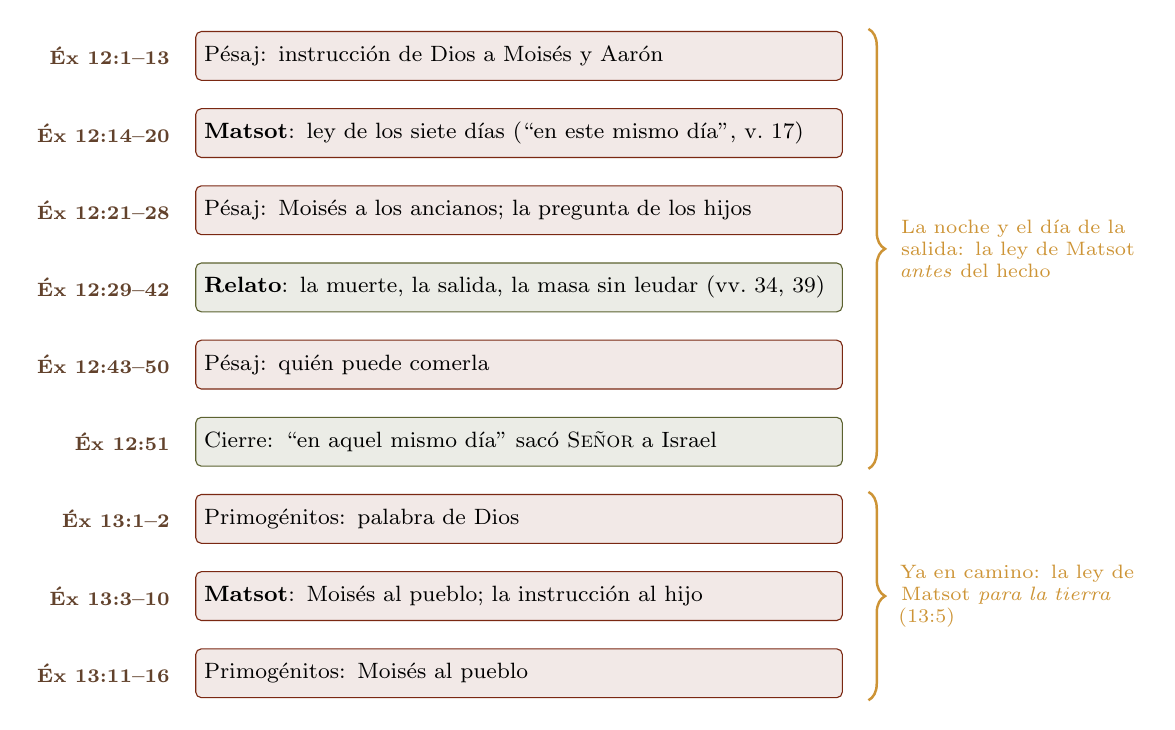
\begin{tikzpicture}[font=\small,x=1cm,y=-0.98cm]
 \tikzset{ley/.style={draw=tierraroja,fill=tierraroja!10,rounded corners=2pt,text width=8.0cm,minimum height=0.62cm,inner sep=3pt,font=\footnotesize},
          rel/.style={draw=oliva,fill=oliva!12,rounded corners=2pt,text width=8.0cm,minimum height=0.62cm,inner sep=3pt,font=\footnotesize},
          ref/.style={font=\scriptsize\bfseries,text=sepia,anchor=east}}
 \foreach \y/\r/\t/\s in {0/{12:1--13}/{Pésaj: instrucción de Dios a Moisés y Aarón}/ley,
                          1/{12:14--20}/{\textbf{Matsot}: ley de los siete días (``en este mismo día'', v.~17)}/ley,
                          2/{12:21--28}/{Pésaj: Moisés a los ancianos; la pregunta de los hijos}/ley,
                          3/{12:29--42}/{\textbf{Relato}: la muerte, la salida, la masa sin leudar (vv.~34, 39)}/rel,
                          4/{12:43--50}/{Pésaj: quién puede comerla}/ley,
                          5/{12:51}/{Cierre: ``en aquel mismo día'' sacó \SENOR{} a Israel}/rel,
                          6/{13:1--2}/{Primogénitos: palabra de Dios}/ley,
                          7/{13:3--10}/{\textbf{Matsot}: Moisés al pueblo; la instrucción al hijo}/ley,
                          8/{13:11--16}/{Primogénitos: Moisés al pueblo}/ley}{
   \node[\s,anchor=west] (n\y) at (2.2,\y) {\t};
   \node[ref] at (2.0,\y) {Éx \r};}
 \draw[decorate,decoration={brace,amplitude=6pt},mostaza!90!tierraroja,line width=0.9pt] (10.75,-0.35) -- (10.75,5.35) node[midway,right=8pt,font=\scriptsize,text width=3.0cm,align=left]{La noche y el día de la salida: la ley de Matsot \emph{antes} del hecho};
 \draw[decorate,decoration={brace,amplitude=6pt},mostaza!90!tierraroja,line width=0.9pt] (10.75,5.65) -- (10.75,8.35) node[midway,right=8pt,font=\scriptsize,text width=3.0cm,align=left]{Ya en camino: la ley de Matsot \emph{para la tierra} (13:5)};
\end{tikzpicture}\par\nopagebreak
{\footnotesize\color{sepia}\textit{Figura 6.} La alternancia de ley y relato en Éxodo 12:1--13:16. \textit{Nota.} Elaboración propia; en rojo, leyes; en verde, relato.}
\end{minipage}\end{center}

La disposición tiene un efecto sobre el lector, que oye la ley de los siete días (12:14--20) antes de ver a los israelitas con la masa al hombro (12:34), y la oye otra vez (13:3--10) cuando ya están en camino. La primera vez la ley anticipa; la segunda, recuerda; entre ambas, el relato pone la prueba de que lo que se mandó comer es lo que de hecho se comió. Y en el centro está la pregunta de los hijos, ``¿Qué es este rito vuestro?'' (12:26), con su respuesta en 13:8: ``Se hace esto con motivo de lo que \SENOR{} hizo conmigo cuando me sacó de Egipto''. La fiesta está pensada como catequesis familiar.

\subsection{Lot, Abraham y el pan sin levadura}
El documento de referencia lee Gn 18--19 como prueba de que la fiesta existía antes de Sinaí, en el ``período tácito de la ley'': Lot ofrece a los ángeles panes sin levadura (\heb{וּמַצּוֹת אָפָה}, ``y coció \emph{matsot}'', Gn 19:3), porque era el tiempo de la fiesta; Abraham, en cambio, no se los ofrece (Gn 18:6--8), ``porque no era aún época de consumirlos''.

\begin{nota}[Precisión: lectura de la serie]
La observación es antigua: Rashi comenta Gn 19:3 con dos palabras, ``era Pésaj'', aunque la tradición rabínica sitúa también la visita a Abraham en Pésaj. El texto hebreo, por su parte, no dice que Abraham ofreciera pan leudado: Sara hace \emph{ugot} (``tortas''), sin indicar si llevaban levadura, y las dos escenas ocurren el mismo día (Gn 19:1, ``a la caída de la tarde''). La \emph{matsá} era además el pan de la hospitalidad apurada (Jue 6:19; 1~S 28:24). La lectura de la serie es posible como eco, y así la expongo; el texto no la hace explícita.
\end{nota}

\subsection{La levadura como metáfora: la Biblia interpreta la Biblia}
Fuera de la cocina, la levadura funciona en la Escritura como imagen de lo pequeño que transforma lo grande, y su sentido depende de qué es lo que se esparce.

\begin{center}\begin{minipage}{\linewidth}\centering
\begin{tikzpicture}[font=\small]
 \node[draw=caferojizo,line width=1pt,fill=papiro,circle,minimum size=2.4cm,align=center,font=\small\bfseries,text=tierraroja] (c) at (0,0) {Levadura\\ \grc{ζύμη}\\ \heb{שְׂאֹר}};
 \node[draw=tierraroja,fill=tierraroja!8,rounded corners=3pt,text width=5.2cm,inner sep=5pt,anchor=east,font=\small] (n) at (-2.2,1.45) {\textbf{\textcolor{tierraroja}{Lo que corrompe}}\\[2pt]
   doctrina de fariseos y saduceos (Mt 16:6, 12)\\ hipocresía (Lc 12:1)\\ la de Herodes (Mc 8:15)\\ malicia y maldad (1~Co 5:8)\\ el error que se esparce (Gá 5:9)};
 \node[draw=oliva,fill=oliva!10,rounded corners=3pt,text width=5.2cm,inner sep=5pt,anchor=west,font=\small] (p) at (2.2,1.45) {\textbf{\textcolor{oliva!80!black}{Lo que crece}}\\[2pt]
   el reino de los cielos, escondido en tres medidas de harina ``hasta que todo fue leudado'' (Mt 13:33; Lc 13:20--21)};
 \node[draw=sepia,fill=mostaza!12,rounded corners=3pt,text width=5.2cm,inner sep=5pt,anchor=east,font=\small] (a) at (-2.2,-1.5) {\textbf{\textcolor{sepia}{Excluida del altar y de la fiesta}}\\[2pt]
   Lv 2:11; 6:17; Éx 12:15--20; 23:18; 34:25};
 \node[draw=sepia,fill=mostaza!12,rounded corners=3pt,text width=5.2cm,inner sep=5pt,anchor=west,font=\small] (b) at (2.2,-1.5) {\textbf{\textcolor{sepia}{Ordenada en la mesa}}\\[2pt]
   acción de gracias (Lv 7:13); dos panes de Shavuot (Lv 23:17)};
 \foreach \x in {n,p,a,b} \draw[mostaza!90!tierraroja,line width=1.1pt] (c) -- (\x);
\end{tikzpicture}\par\nopagebreak
{\footnotesize\color{sepia}\textit{Figura 7.} La levadura en la Biblia: usos negativos, positivos y rituales. \textit{Nota.} Elaboración propia.}
\end{minipage}\end{center}

En boca de Jesús la levadura es primero una advertencia. Cuando los discípulos olvidan el pan, les dice: ``Mirad, guardaos de la levadura de los fariseos y de los saduceos'' (Mt 16:6); ellos piensan en el pan, hasta que ``entendieron que no les había dicho que se guardasen de la levadura del pan, sino de la doctrina de los fariseos y de los saduceos'' (16:12). Lucas precisa: ``la levadura de los fariseos, que es la hipocresía'' (Lc 12:1). La enseñanza falsa y la apariencia sin verdad actúan como la masa madre, invisibles al principio y presentes al final en toda la masa.

La misma imagen sirve, sin embargo, para el reino: ``El reino de los cielos es semejante a la levadura que tomó una mujer, y escondió en tres medidas de harina, hasta que todo fue leudado'' (Mt 13:33). Aquí la levadura es buena, porque lo que se esparce es el reino. Las ``tres medidas'' (\grc{σάτα τρία}) recuerdan las ``tres medidas de flor de harina'' (\heb{שְׁלֹשׁ סְאִים}) que Sara amasa para los visitantes de Dios (Gn 18:6), y el documento de referencia las lee como las tres etapas de la Iglesia (primogénitos, Israel, Iglesia del Nuevo Pacto). Sea cual sea la aplicación, la parábola impide convertir la levadura en un símbolo fijo del mal. La levadura significa lo que el contexto dice que se esparce: en la fiesta de la salida se quita la vieja masa de Egipto; en el reino, lo que leuda es la vida nueva.

\subsection{Cuatro levaduras en el Nuevo Testamento}
En mi presentación anterior sobre los Panes sin Levadura ordené los usos negativos de la imagen en el Nuevo Testamento según quién la esparce. Son cuatro, y cada una tiene un contenido preciso.

\begin{center}\begin{minipage}{\linewidth}\centering\small\renewcommand{\arraystretch}{1.22}
\begin{tabular}{@{}L{2.6cm}L{6.4cm}L{6.6cm}@{}}
\toprule
\textbf{Levadura} & \textbf{Qué es según el contexto} & \textbf{Textos} \\ \midrule
de Herodes & el poder político que manipula lo religioso, mata al profeta y teme al rey verdadero & Mc 8:14--15; cf. 6:14--18; Mt 2:7--12 \\
de los fariseos & la hipocresía: una religión de apariencia, que dice y no hace & Lc 12:1; Mt 16:5--12; 23:1--3; Lc 11:37--44 \\
de los saduceos & una doctrina que niega lo que Dios puede hacer: la resurrección y los ángeles & Mt 16:6--12; cf. 22:23; Hch 23:8 \\
de Corinto & la inmoralidad tolerada y la jactancia que se infla & 1~Co 4:18--21; 5:1--13; 6:9--20; 8:1; 13:4; 2~Co 12:20--21 \\
\bottomrule
\end{tabular}\par\nopagebreak
{\footnotesize\color{sepia}\textit{Tabla 4.} Las levaduras del Nuevo Testamento. \textit{Nota.} Elaboración propia a partir de mi presentación anterior ``Los Panes sin Levadura''.}
\end{minipage}\end{center}

El cuadro muestra que la ``levadura'' del Nuevo Testamento no es un pecado genérico, sino cada vez algo que se introduce en una comunidad y la transforma desde dentro: una alianza con el poder, una piedad fingida, una enseñanza que achica a Dios, una conducta que la iglesia tolera con orgullo. Al menos tres de ellas comparten un rasgo, la hinchazón. Pablo dice de los corintios que están ``envanecidos'' (\grc{πεφυσιωμένοι}, 1~Co 4:18--19; 5:2) y que ``el conocimiento envanece'' (8:1); el verbo \grc{φυσιόω} es ``inflar'', lo mismo que la levadura hace con la masa. Filón había observado ya que la levadura se excluye del altar porque hace crecer la masa, imagen de la soberbia (cf. \emph{Spec.} 1.293).

La familia hebrea de \emph{jamets} da todavía un eco que recogí en aquella presentación al citar Is 63:1--9. El guerrero que viene de Edom tiene los vestidos \heb{חֲמוּץ בְּגָדִים} (\emph{jamuts begadim}), ``rojos'', teñidos como de lagar (63:1--3); el Apocalipsis retoma la escena en la vendimia de la ira (Ap 14:18--20) y en el jinete ``vestido de una ropa teñida en sangre'' (Ap 19:13). El adjetivo viene de la misma raíz que ``leudado'', aquí con el sentido de color intenso. El vínculo es de raíz y no de sentido, y por eso lo presento como eco.

\subsection{1 Corintios 5:6--8: estructura de un argumento}
Pablo recurre a la fiesta para resolver un caso de inmoralidad tolerada en la iglesia de Corinto (1~Co 5:1--5), y su argumento sigue el orden de la cocina de la Pascua.

\par\smallskip{\centering\large\grc{ἐκκαθάρατε τὴν παλαιὰν ζύμην, ἵνα ἦτε νέον φύραμα, καθώς ἐστε ἄζυμοι.}\\ \grc{καὶ γὰρ τὸ πάσχα ἡμῶν ἐτύθη Χριστός.}\par}\smallskip
\begin{cita}No es buena vuestra jactancia. ¿No sabéis que un poco de levadura leuda toda la masa? Limpiaos, pues, de la vieja levadura, para que seáis nueva masa, sin levadura como sois; porque nuestra pascua, que es Cristo, ya fue sacrificada por nosotros. Así que celebremos la fiesta, no con la vieja levadura, ni con la levadura de malicia y de maldad, sino con panes sin levadura, de sinceridad y de verdad.\fuente{(1~Co 5:6--8)}\end{cita}

\begin{center}\begin{minipage}{\linewidth}\centering
\begin{tikzpicture}[font=\small,node distance=0.32cm]
 \tikzset{b/.style={draw=tierraroja,fill=papiro,rounded corners=3pt,text width=10.0cm,inner sep=4pt,font=\small},
          lab/.style={font=\scriptsize\bfseries,text=papiro,fill=tierraroja,rounded corners=2pt,inner sep=3pt,text width=2.3cm,align=center}}
 \node[b] (a) {``Un poco de levadura leuda toda la masa'' (\grc{μικρὰ ζύμη ὅλον τὸ φύραμα ζυμοῖ}): el peligro del contagio};
 \node[b,below=of a] (b2) {``Limpiaos de la vieja levadura'' (\grc{ἐκκαθάρατε}, aoristo: una limpieza decisiva), ``para que seáis nueva masa''};
 \node[b,below=of b2] (c) {``Sin levadura como sois'' (\grc{καθώς ἐστε ἄζυμοι}): lo que ya son en Cristo};
 \node[b,below=of c,fill=tierraroja!12] (d) {``Porque nuestra pascua, que es Cristo, ya fue sacrificada'' (\grc{ἐτύθη}, aoristo pasivo): el hecho que lo funda todo};
 \node[b,below=of d] (e) {``Celebremos la fiesta'' (\grc{ἑορτάζωμεν}, presente: sigamos celebrando) \textbf{no con} levadura vieja, malicia y maldad, \textbf{sino con} ázimos de sinceridad y de verdad};
 \foreach \n/\t in {a/{Proverbio (v.~6b)},b2/{Imperativo (v.~7a)},c/{Indicativo (v.~7a)},d/{Fundamento (v.~7b)},e/{Exhortación (v.~8)}}
   \node[lab,left=0.25cm of \n] {\t};
 \draw[-{Latex[length=2.5mm]},mostaza!90!tierraroja,line width=1.2pt] (d.east) .. controls +(1.2,0) and +(1.2,0) .. (b2.east) node[midway,right,font=\scriptsize\itshape,text=sepia,text width=1.6cm]{el sacrificio precede a la limpieza};
\end{tikzpicture}\par\nopagebreak
{\footnotesize\color{sepia}\textit{Figura 8.} Estructura de 1~Corintios 5:6--8. \textit{Nota.} Elaboración propia con NA28.}
\end{minipage}\end{center}

El orden es el de Éxodo: primero se sacrifica el cordero, después se come el pan sin levadura durante siete días. Pablo no dice ``quitad la levadura para que Cristo sea sacrificado'', sino ``quitad la levadura, porque Cristo ya fue sacrificado''; el imperativo descansa en el indicativo, ``sed lo que sois''. La ``vieja levadura'', además, es un pecado concreto, el que la comunidad tolera y que, como la masa madre guardada, contamina la amasada siguiente. Por eso Pablo pide expulsar al que vive en inmoralidad (5:13, citando la fórmula de Dt 17:7: ``quitad, pues, a ese perverso de entre vosotros'').

%===================================================================
\section{Memorial, figura y esperanza: la lectura de la serie}

\subsection{El marco: el reglamento del culto}
El documento de referencia de la serie lee Levítico 23 como el ``reglamento del culto'': las solemnidades del \SENOR{} proclamadas ``santas convocaciones'' o ``citaciones santas'', fijadas ``en sus tiempos'' y dadas ``por estatuto perpetuo''. Cada fiesta es a la vez memorial de un hito de la historia de Israel y figura de una etapa del plan de salvación. Para la fiesta de los Ázimos el documento fija cuatro rasgos: es memorial perpetuo del día en que Israel salió de Egipto; dentro de ella se presenta el \emph{ómer} que identifica a Israel como primicia de las naciones; su primer y su último día son santos; y durante los siete días se comen panes sin levadura.

\begin{center}\begin{minipage}{\linewidth}\centering\small\renewcommand{\arraystretch}{1.25}
\begin{tabular}{@{}L{4.6cm}L{2.6cm}L{8.4cm}@{}}
\toprule
\textbf{Hito de Israel} & \textbf{Fiesta} & \textbf{Nuevo Pacto (lectura de la serie)} \\ \midrule
Salvado de la muerte de los primogénitos (Éx 12:13) & Pascua, 14 & Cristo nuestra Pascua (1~Co 5:7); la Cena, memorial ``hasta que él venga'' \\
\textbf{Salida de Egipto} (Éx 12:17) & \textbf{Ázimos, 15--21} & \textbf{La Iglesia sin levadura de pecado, libre del dominio de Satanás} (1~Co 5:7--8); los apóstoles la observan (Hch 12:3; 20:6) \\
Libre del faraón tras el mar, ``18 de Abib'' (Éx 19:5--6) & Primicias & Cristo, primicia de los resucitados (1~Co 15:20--23) \\
\bottomrule
\end{tabular}\par\nopagebreak
{\footnotesize\color{sepia}\textit{Tabla 5.} Las fiestas de primavera en la lectura de la serie. \textit{Nota.} Elaboración propia a partir del documento de referencia (lecciones 7 y 11).}
\end{minipage}\end{center}

\subsection{Egipto, el faraón e Israel}
La lección 11 del documento desarrolla la figura mediante correspondencias: ``Egipto, el Faraón, Israel cautivo, el Cordero que se sacrificaba en la Pascua del Antiguo Pacto simbolizaban respectivamente al Mundo, a Satanás, a la Iglesia, a Nuestro Señor crucificado en el Nuevo Pacto''. Así como Israel fue esclavo en Egipto, la Iglesia ``en el Egipto del mundo, estaba presa de Satanás''; así como los hebreos estaban bajo pena de muerte, los creyentes estaban ``muertos en delitos y pecados''. La serie apoya la figura en Efesios 2:

\begin{cita}Y él os dio vida a vosotros, cuando estabais muertos en vuestros delitos y pecados, en los cuales anduvisteis en otro tiempo, siguiendo la corriente de este mundo, conforme al príncipe de la potestad del aire, el espíritu que ahora opera en los hijos de desobediencia\ldots\fuente{(Ef 2:1--2)}\end{cita}

En esa lectura, la ``masa sin levadura'' que los israelitas llevaban el día de su liberación representa ``la marcha de la Iglesia liberada de la levadura del pecado''. La Pascua salva de la muerte; los Ázimos sacan del dominio del opresor. De ahí concluye el documento que la Pascua quedó transformada en memorial del sacrificio de Cristo, mientras que los Ázimos, cuyo universo simbólico ``era mucho más amplio en el tiempo'', siguen siendo una conmemoración perpetua para el pueblo de Dios, observada por la Iglesia de los apóstoles después de la muerte del Señor.

La figura tiene apoyos dentro de la Escritura:
\begin{itemize}\setlength{\itemsep}{1pt}
\item Pablo lee el éxodo como figura de la Iglesia: ``todos nuestros padres estuvieron bajo la nube, y todos pasaron el mar\ldots{} Y estas cosas sucedieron como ejemplos para nosotros'' (1~Co 10:1, 6; \grc{τύποι}, ``tipos'').
\item El Nuevo Testamento describe la salvación como un éxodo de un dominio a otro: Dios ``nos ha librado de la potestad de las tinieblas, y trasladado al reino de su amado Hijo'' (Col 1:13); Cristo vino a ``destruir por medio de la muerte al que tenía el imperio de la muerte, esto es, al diablo, y librar a todos los que\ldots{} estaban durante toda la vida sujetos a servidumbre'' (He 2:14--15).
\item Los profetas ya habían presentado al faraón con rasgos de monstruo: ``el gran dragón que yace en medio de sus ríos'' (Ez 29:3), y la victoria del mar como victoria sobre Rahab, el dragón (Is 51:9--10). El Apocalipsis llama a Satanás ``el gran dragón'' (Ap 12:9).
\item Jesús define la esclavitud en términos de pecado: ``todo aquel que hace pecado, esclavo es del pecado'' (Jn 8:34).
\end{itemize}

\begin{nota}[Precisión]
Las correspondencias Egipto = mundo, faraón = Satanás, Israel = Iglesia son lectura tipológica de la serie, con apoyos intra-bíblicos reales (1~Co 10:1--11; Col 1:13; He 2:14--15; Ez 29:3; Ap 12:9). Ningún texto dice explícitamente ``el faraón es Satanás''. La lectura de la ``masa sin levadura'' como Iglesia sin pecado se apoya en 1~Co 5:7 (``sin levadura como sois''). La relación del ``18 de Abib'' con el \emph{ómer} pertenece al estudio de las Primicias y depende de la cronología discutida en la sección~3.5. El documento atribuye Hebreos a Pablo; como la autoría de Hebreos es discutida, aquí lo cito como Escritura sin asignarle autor.
\end{nota}

\subsection{La observancia apostólica}
El documento presenta tres textos del Nuevo Testamento como prueba de que la Iglesia apostólica guardó la fiesta.

\paragraph{Hechos 12:3.} ``Y viendo que esto había agradado a los judíos, procedió a prender también a Pedro. Eran entonces los días de los panes sin levadura''. El documento infiere que Herodes ``sabía que en ese día iba a encontrar a los que perseguía'', porque la consagración de esos días ``era un mandato de ley que la Iglesia iba a cumplir''. El texto dice menos. Lucas fecha el arresto por la fiesta y añade que Herodes quería presentar a Pedro al pueblo ``después de la pascua'' (12:4); la fecha muestra que la Iglesia de Jerusalén vivía dentro del calendario de las fiestas, y el motivo de Herodes que Lucas da es agradar a los judíos.

\paragraph{Hechos 20:6.} ``Y nosotros, pasados los días de los panes sin levadura, navegamos de Filipos''. Pablo y Lucas permanecen en Filipos durante la fiesta y solo después zarpan. Comentaristas como Longenecker (1981) entienden que Pablo, sin poder llegar a Jerusalén, celebró allí la Pascua y los Ázimos; otros ven solo una indicación de calendario. Que esperaran hasta el fin de los siete días pesa a favor de la observancia.

\paragraph{1 Corintios 5:8.} ``Así que celebremos la fiesta''. Es el texto central y se discute en la sección~\ref{sec:discusion}. Para la serie, Pablo se refiere ``explícitamente a la misma fiesta que Dios había instituido'' (Iglesia de Dios Unida, 2011), y la comunidad de Corinto, judíos y gentiles, la guardaba físicamente; Pablo usa esa práctica para enseñar su sentido.

\subsection{Mi presentación anterior: la casa sin levadura}
Cuando preparé las láminas de esta fiesta (``Los Panes sin Levadura'') la situé en el ciclo agrícola de Israel y la leí en tres planos: la fiesta, sus cumplimientos históricos y sus sombras proféticas. Tres de aquellos énfasis completan la lectura de la serie.

\paragraph{La búsqueda de la levadura.} Partí de la práctica judía de la \emph{bedikat jamets}: antes de la Pascua la casa se limpia hasta el último rincón. La aplicación es bíblica, porque los creyentes son ``casa'' de Dios (He 3:6; 1~Ti 3:15; Ef 2:19), ``piedras vivas'' de una ``casa espiritual'' (1~P 2:5), y su cuerpo es ``templo del Espíritu Santo'' (1~Co 6:19; cf. 3:16--17; 2~Co 6:16). Si la casa de Israel debía quedar sin \emph{se'or}, la casa de Dios debe quedar sin la levadura del pecado. La búsqueda nocturna con lámpara es tradición (Pesajim 1:1); la imagen de la casa de Dios es de la Escritura.

\paragraph{El gran sábado.} La semana de la Pascua tiene un día de reposo propio, el 15 de Nisán, además del sábado semanal: es el ``gran'' día de Jn 19:31 (``aquel día de reposo era de gran solemnidad''), coherente con Lv 23:7 (\emph{mikrá kódesh}, sin trabajo servil).

\paragraph{Cómo celebrarla hoy.} La respuesta es la de 1~Co 5:8, ``con sinceridad y verdad'', es decir, con pureza, santidad y separación, a la que añadí el lavamiento: ``ya habéis sido lavados, ya habéis sido santificados'' (1~Co 6:11); ``levántate y bautízate, y lava tus pecados'' (Hch 22:16). Pablo había leído el paso del mar, que sigue a la Pascua, como bautismo: ``todos en Moisés fueron bautizados en la nube y en el mar'' (1~Co 10:2). La salida de Egipto termina en el agua, y la vida sin levadura se alimenta de la Palabra en la que el creyente se sumerge.

\begin{nota}[Precisión: el 17 de Nisán]
En aquella presentación reuní en el 17 de Nisán varios hechos: el arca que reposa sobre el Ararat (Gn 8:4, ``en el mes séptimo, a los diecisiete días'', leído según el calendario civil que comenzaba en Tishri, de modo que el séptimo mes sería Nisán), el cruce del mar, el primer fruto de la tierra (Jos 5:10--12) y la caída de Amán (Est 3--7). Son cómputos tradicionales. Gn 8:4 solo dice ``mes séptimo''; el cruce del mar no tiene fecha en el texto (sección~3.5); Jos 5:11 dice ``al otro día de la pascua'', es decir, el 15; en Ester, el edicto se escribe el 13 del primer mes (Est 3:12) y el banquete y la caída de Amán se sitúan tradicionalmente dos o tres días después, sin fecha explícita en el texto. Pueden usarse como ecos, no como datos.
\end{nota}

\subsection{Los materiales de la serie}
El folleto \emph{Las fiestas santas de Dios} (Iglesia de Dios Unida, 2011), que forma parte de los materiales del proyecto, desarrolla la misma lectura con énfasis práctico: la fiesta enseña a ``salir del pecado''; sacar la levadura de la casa durante siete días recuerda que hay que reconocer, expulsar y evitar el pecado; la semana es tiempo de examen (2~Co 13:5) y de victoria sobre el pecado por la ayuda de Dios (Ro 7:21--25; Fil 2:12--13). Otro material del proyecto, \emph{El poder espiritual de las siete fiestas de Dios}, lee la \emph{matsá} como figura del cuerpo de Cristo, sin pecado, y la sepultura de Jesús como cumplimiento de la fiesta, lectura que se discute en la sección~\ref{sec:mesias}.

%===================================================================
\section{La fiesta en Jesús y los apóstoles}\label{sec:mesias}

\subsection{``Yo soy el pan de vida''}
El evangelio de Juan sitúa el gran discurso del pan en el calendario de la fiesta: ``Y estaba cerca la pascua, la fiesta de los judíos'' (Jn 6:4). Jesús alimenta a cinco mil, cruza el mar, y en la sinagoga de Capernaúm compara su obra con el maná del desierto:

\par\smallskip{\centering\large\grc{ἐγώ εἰμι ὁ ἄρτος τῆς ζωῆς}\par}\smallskip
\begin{cita}Yo soy el pan de vida; el que a mí viene, nunca tendrá hambre; y el que en mí cree, no tendrá sed jamás.\fuente{(Jn 6:35)}\end{cita}
\begin{cita}Yo soy el pan de vida. Vuestros padres comieron el maná en el desierto, y murieron. Este es el pan que desciende del cielo, para que el que de él come, no muera. Yo soy el pan vivo que descendió del cielo; si alguno comiere de este pan, vivirá para siempre; y el pan que yo daré es mi carne, la cual yo daré por la vida del mundo.\fuente{(Jn 6:48--51)}\end{cita}

El discurso habla del maná y no de la \emph{matsá}, pero el escenario es el de la Pascua y los Ázimos, y la secuencia (comida en el desierto, paso del mar, pan del cielo) reproduce el éxodo. Jesús se presenta como el pan que da la vida que ni el pan de Egipto ni el del desierto daban: el pan de aflicción recordaba la salida; el pan de vida la cumple.

\subsection{``Esto es mi cuerpo''}
En la última cena Jesús ``tomó el pan y dio gracias, y lo partió y les dio, diciendo: Esto es mi cuerpo, que por vosotros es dado; haced esto en memoria de mí'' (Lc 22:19). Si la cena fue la comida pascual, como presentan los sinópticos (Mc 14:12--16; Lc 22:7--15), el pan que Jesús partió era \emph{matsá}, pan de aflicción, y el ``haced esto en memoria de mí'' retoma el ``os será en memoria'' de Éx 12:14 (Jeremias, 1966). El texto griego dice \grc{ἄρτος} (``pan''), palabra general que la LXX usa también para los ázimos (\grc{ἄρτους ἀζύμους}, Éx 29:2), así que la terminología no decide la cuestión. El documento de la serie lee la cena como la última Pascua de Jesús, reinstalada como memorial ``hasta que él venga'' (1~Co 11:26).

\begin{nota}[Precisión]
La fecha de la cena es un problema clásico. Los sinópticos la presentan como comida pascual; Juan sitúa la crucifixión el día de la ``preparación de la pascua'' (Jn 18:28; 19:14), cuando se sacrificaban los corderos. Se han propuesto calendarios distintos, una cena pascual anticipada o una cena no pascual con rasgos pascuales (Jeremias, 1966, defiende el carácter pascual). Mil años después, la cuestión del pan alimentó la controversia entre la Iglesia latina, que usaba ázimos en la eucaristía, y la griega, que usaba pan leudado (siglo~\textsc{xi}); es historia posterior y no decide el sentido bíblico.
\end{nota}

\subsection{La sepultura en los días de los ázimos}
Juan precisa que los judíos pidieron bajar los cuerpos antes de la tarde ``por cuanto era la preparación de la pascua\ldots{} (pues aquel día de reposo era de gran solemnidad)'' (Jn 19:31): \grc{ἦν γὰρ μεγάλη ἡ ἡμέρα ἐκείνου τοῦ σαββάτου}. El ``gran'' sábado es el 15 de Nisán, primer día santo de los Ázimos, de modo que Jesús fue sepultado al caer el sol, cuando comenzaba la fiesta. El material \emph{El poder espiritual de las siete fiestas} lo lee como cumplimiento: el cuerpo sin pecado, el ``grano de trigo'' que cae en tierra (Jn 12:24), sepultado en el día de la fiesta del pan sin levadura.

\begin{nota}[Precisión]
Que Jesús fue sepultado al comenzar el 15 de Nisán se sigue de Jn 19:31, 42. El día de la semana es discutido: la tradición mayoritaria sostiene el viernes; algunas corrientes, entre ellas la que siguen ciertos materiales del proyecto, proponen el miércoles, para contar tres días y tres noches completos (Mt 12:40), con dos sábados en esa semana (el de la fiesta y el semanal). Las lecturas devocionales de la \emph{matsá} actual, ``rayada y perforada'' como imagen de Is 53:5 y Zac 12:10, describen la forma moderna del pan (las perforaciones evitan que la masa se infle) y el rito medieval del \emph{afikomán}; son aplicaciones posteriores, no datos del texto.
\end{nota}

\subsection{Pablo: la fiesta y la vida}
En 1~Co 5:6--8 Pablo usa la fiesta en dos niveles. En el del calendario, el pasaje supone que los corintios conocen la cocina de la Pascua, la levadura vieja, la limpieza de la casa, la masa nueva, el cordero sacrificado; la carta se escribió desde Éfeso, donde Pablo pensaba quedarse ``hasta Pentecostés'' (1~Co 16:8), lo que sugiere una fecha de primavera, cerca de la Pascua (Fee, 1987; Hays, 1997). En el nivel moral, la fiesta describe la vida de la comunidad: ``celebremos la fiesta\ldots{} con panes sin levadura, de sinceridad y de verdad''. El mismo proverbio de la levadura reaparece en Gálatas, ``Un poco de levadura leuda toda la masa'' (Gá 5:9), dicho de la enseñanza que obligaba a los gentiles a circuncidarse.

\subsection{El éxodo en el Nuevo Testamento}
La fiesta pertenece a un tema más amplio del Nuevo Testamento. Lucas llama ``éxodo'' (\grc{ἔξοδος}) a la muerte de Jesús en Jerusalén (Lc 9:31); Pedro escribe a los creyentes ``ceñid los lomos de vuestro entendimiento'' (1~P 1:13), con la ropa de la noche de la Pascua (Éx 12:11), y los llama ``rescatados\ldots{} con la sangre preciosa de Cristo, como de un cordero sin mancha'' (1~P 1:18--19); el Apocalipsis pone en boca de los vencedores ``el cántico de Moisés siervo de Dios, y el cántico del Cordero'' (Ap 15:3). Dentro de ese éxodo, el pan sin levadura es la parte que dura, la vida del que ya salió.

%===================================================================
\section{La fiesta en la tradición judía}\label{sec:tradicion}

\begin{nota}[Precisión]
Esta sección describe la práctica judía posterior, codificada en la Misná (ca. 200 e.\,c.), el Talmud y la liturgia. Se expone como tradición, no como norma bíblica, aunque muchas de sus prácticas reflejan el Segundo Templo.
\end{nota}

\paragraph{La búsqueda y la quema.} ``La noche del catorce se busca el \emph{jamets} a la luz de una lámpara'' (Misná Pesajim 1:1), la \emph{bedikat jamets}. Al día siguiente, la Misná fija hasta qué hora puede comerse lo leudado y cuándo debe quemarse (Pesajim 1:4; 2:1), la \emph{biur jamets}. La práctica posterior añade una fórmula aramea de anulación (\emph{kol jamirá}), por la que el dueño declara sin valor cualquier levadura que no haya encontrado.

\paragraph{La \emph{matsá}.} Solo cinco cereales sirven para cumplir el precepto de la \emph{matsá}: trigo, cebada y otros tres tradicionalmente identificados con la espelta, el centeno y la avena (Pesajim 2:5). Lo que cuenta como \emph{jamets} es la masa de esos cereales que fermenta; la tradición posterior fijó el límite en unos dieciocho minutos desde que la harina toca el agua, derivado del tiempo de recorrer un \emph{mil} (Pesajim 46a). Los más estrictos comen \emph{matsá shemurá}, ``vigilada'' desde la siega, por la lectura literal de Éx 12:17 (``vigilaréis las \emph{matsot}'').

\paragraph{La noche del Séder.} La Misná prescribe la comida de la noche del 15 y su relato (Pesajim 10). Rabán Gamaliel enseña que quien no explica tres cosas no ha cumplido: el sacrificio de Pésaj, la \emph{matsá} y las hierbas amargas; la \emph{matsá}, ``porque nuestros padres fueron redimidos'' (Pesajim 10:5). La forma actual del Séder y de la Hagadá es posterior (Bokser, 1984).

\paragraph{Los días de la fiesta.} Los días intermedios se llaman \emph{jol hamoed}; el séptimo, \emph{shevi'i shel Pésaj}, se dedica al recuerdo del mar con la lectura de Éx 13:17--15:26 (Meguilá 31a). Fuera de la tierra de Israel la tradición rabínica añade un octavo día, por la antigua incertidumbre en la fijación del calendario.

\paragraph{La lectura moral.} El Talmud conoce la levadura como imagen del impulso al mal: un rabino pide a Dios que quite ``la levadura de la masa'' que impide hacer su voluntad (Berajot 17a). La metáfora de Jesús y Pablo tenía, pues, terreno común en el judaísmo de su época y posterior.

%===================================================================
\section{Discusión de interpretaciones}\label{sec:discusion}

\subsection{1 Corintios 5:8: ¿mandato de guardar la fiesta o metáfora de la vida cristiana?}
El exhortativo \grc{ἑορτάζωμεν} (``celebremos la fiesta'', presente de subjuntivo) admite tres lecturas.

\begin{center}\begin{minipage}{\linewidth}\centering\small\renewcommand{\arraystretch}{1.25}
\begin{tabular}{@{}L{3.3cm}L{6.6cm}L{5.7cm}@{}}
\toprule
\textbf{Lectura} & \textbf{Argumentos} & \textbf{Autores} \\ \midrule
Metáfora de la vida cristiana & El contexto es disciplinario (5:1--13); el presente indica una acción continua (``sigamos celebrando''): toda la vida es la fiesta que sigue a la Pascua; ``levadura'' y ``ázimos'' están calificados moralmente (malicia, sinceridad) & Fee (1987); Thiselton (2000) \\
Observancia literal con sentido nuevo & Pablo escribe cerca de la Pascua (16:8); la imagen supone la práctica de limpiar la casa; Hch 20:6 muestra a Pablo deteniéndose durante los Ázimos; ``celebremos'' es una exhortación a celebrar & Bacchiocchi (1995); Iglesia de Dios Unida (2011); documento de la serie \\
Lectura combinada & La metáfora nace de una práctica viva: la comunidad conocía la fiesta y Pablo da a su cocina un contenido ético y cristológico, sin legislar en el pasaje sobre su observancia & Hays (1997) \\
\bottomrule
\end{tabular}\par\nopagebreak
{\footnotesize\color{sepia}\textit{Tabla 6.} Lecturas de 1~Co 5:8. \textit{Nota.} Elaboración propia.}
\end{minipage}\end{center}

Fee sostiene que, para Pablo, la Pascua ya se cumplió en la muerte de Cristo y que la vida de la iglesia es la fiesta continua de los ázimos, sin referencia al calendario anual; Thiselton desarrolla la misma idea a partir del tiempo verbal y de la oposición ``vieja levadura / masa nueva''. Bacchiocchi, desde una lectura sabatista, observa que la metáfora sería poco comprensible para una iglesia que no conociera la práctica, y que Pablo no les pide dejar de observar la fiesta, sino observarla con su sentido en Cristo. La serie sigue esta segunda línea. Lo que las tres lecturas tienen en común sí lo sostiene el texto: la fiesta tiene su sentido pleno en Cristo, nuestra Pascua, y se celebra con una vida sin malicia. La pregunta por la observancia anual no se decide en este pasaje, sino en el conjunto de los textos (Hch 12:3; 20:6; Col 2:16--17; Ro 14:5--6), que la serie estudia en sus lecciones sobre el Nuevo Pacto.

\subsection{¿Dónde cruzó Israel el mar, y cuándo?}
La geografía (ruta norte por los lagos y lagunas del istmo o ruta sur hacia el golfo de Suez) sigue abierta (Hoffmeier, 1997; Kitchen, 2003), y la cronología también. La serie fija el cruce el 17 de Abib y presenta el 18 como el día de Israel libre del faraón; la tradición rabínica lo fija el 21, séptimo día de la fiesta; el texto solo fecha la salida. Ambas reconstrucciones comparten la convicción de que la semana de los Ázimos conmemora la liberación completa, salida y mar.

\subsection{¿Es la levadura siempre símbolo del pecado?}
Una lectura frecuente identifica la levadura con el mal en toda la Biblia; algunos comentaristas leen así incluso Mt 13:33, como la corrupción que penetra la cristiandad (Scofield, 1909; Pentecost, 1958). La mayoría lee la parábola como imagen del crecimiento del reino desde un comienzo escondido (Davies \& Allison, 1991; Hagner, 1993). Los datos de la Torá (Lv 7:13; 23:17) y la parábola de la mujer favorecen la segunda lectura, en la que la levadura significa lo que se esparce y el contexto dice si es malicia o reino.

\subsection{¿Dos fiestas o una?}
La crítica histórica distingue un origen pastoral de Pésaj y uno agrícola de Matsot (de Vaux, 1985); el texto canónico las presenta unidas desde Éxodo 12 y con un único origen histórico. Ezequiel, Esdras, Josefo y los evangelios las nombran juntas y a veces con un solo nombre. La serie las distingue por su significado (salvación de la muerte, salida del cautiverio) sin separarlas en el tiempo.

%===================================================================
\section{Síntesis}

\begin{tcolorbox}[enhanced,unbreakable,colback=papiro,colframe=tierraroja,boxrule=1pt,arc=3pt,title={Definición},fonttitle=\bfseries,coltitle=papiro,colbacktitle=tierraroja]
La fiesta de los Panes sin Levadura (\heb{חַג הַמַּצּוֹת}, \emph{jag hamatsot}; \grc{ἑορτὴ τῶν ἀζύμων}) es la convocación del \SENOR{} del 15 al 21 de Abib, con el primero y el séptimo día santos, en la que Israel come \emph{matsot} y quita de sus casas toda \emph{se'or} y todo \emph{jamets}, ``porque en este mismo día saqué vuestras huestes de la tierra de Egipto'' (Éx 12:17). Es memorial de la salida (``pan de aflicción, porque aprisa saliste'', Dt 16:3) y, en el Nuevo Testamento, imagen de la comunidad que, porque ``nuestra pascua, que es Cristo, ya fue sacrificada'', vive como ``nueva masa, sin levadura'', ``de sinceridad y de verdad'' (1~Co 5:7--8).
\end{tcolorbox}

\begin{center}\begin{minipage}{\linewidth}\centering\small\renewcommand{\arraystretch}{1.25}
\begin{tabular}{@{}L{3cm}L{12.6cm}@{}}
\toprule
\textbf{Lectura} & \textbf{Aporte a la comprensión de la fiesta} \\ \midrule
Histórica & La fiesta conmemora la salida de prisa: masa sin leudar en las artesas, pan de pobres y de caminantes; se celebró en Gilgal, bajo Ezequías, Josías y Esdras, y en el Segundo Templo, siempre unida a la Pascua. \\
Filológica & El hebreo distingue la masa madre (\emph{se'or}), lo leudado (\emph{jamets}) y el pan sin leudar (\emph{matsá}); \emph{lejem oni} une el pan a la aflicción; \emph{tsiv'ot} presenta al pueblo como hueste de Dios; el griego pasa de \emph{ázyma} a \emph{ázymoi}, personas sin levadura. \\
Textual & El ``primer día'' de quitar la levadura, los ``seis días'' de Dt 16:8, la variante \emph{matsot/mitsvá} de Éx 12:17 y el cómputo de Mc 14:12 muestran una fiesta contada desde la tarde del 14. La levadura está excluida del altar, no de la mesa. \\
Literaria & La semana está encerrada entre dos días santos; la ley está incrustada en el relato del éxodo; la levadura es metáfora de lo que se esparce, para mal (Mt 16:6) o para bien (Mt 13:33). \\
De la serie & Memorial de Israel libre del cautiverio y figura de la Iglesia sin levadura de pecado, libre del dominio de Satanás, observada por los apóstoles (Hch 12:3; 20:6; 1~Co 5:8). \\
En Cristo & Jesús, el pan de vida (Jn 6:35), parte el pan en la cena pascual y es sepultado al comenzar los ázimos (Jn 19:31); Pablo funda la vida sin levadura en su sacrificio (1~Co 5:7). \\
\bottomrule
\end{tabular}\par\nopagebreak
{\footnotesize\color{sepia}\textit{Tabla 7.} Lectura y aporte. \textit{Nota.} Elaboración propia.}
\end{minipage}\end{center}

%===================================================================
\section{Para la reflexión}

\begin{enumerate}
\item Israel comió \emph{matsot} porque salió de prisa, no para poder salir. ¿Qué cambia en la vida cristiana cuando la limpieza de la ``vieja levadura'' se entiende como consecuencia de la Pascua (1~Co 5:7) y no como condición para ella?
\item La ley mandaba quitar la \emph{se'or}, la masa madre, no solo el pan leudado. ¿Cuáles son las ``masas madre'' de la propia vida: hábitos, rencores o enseñanzas que, guardados, fermentan cada nueva amasada?
\item Pablo aplica la fiesta a un pecado que la comunidad toleraba (1~Co 5:1--2). ¿Qué levadura tolera hoy una iglesia por orgullo (``vuestra jactancia'', 5:6)?
\item ``Y lo contarás en aquel día a tu hijo'' (Éx 13:8). ¿Cómo se transmite en la familia el relato de la liberación, de modo que la siguiente generación pueda decir ``lo que el \SENOR{} hizo conmigo''?
\item La levadura del reino crece escondida ``hasta que todo fue leudado'' (Mt 13:33). ¿Dónde se ve en la propia comunidad esa influencia lenta y buena, y cómo se la cuida?
\item El pan de aflicción y el pan de vida: ¿qué significa recordar cada año la pobreza de la que Dios sacó a su pueblo, ``todos los días de tu vida'' (Dt 16:3)?
\end{enumerate}

%===================================================================
\section*{Glosario}\markboth{Glosario}{}
\begin{description}\footnotesize\setlength{\itemsep}{0pt}
\item[Abib] (\heb{אָבִיב}). ``Espiga verde''; nombre del primer mes, llamado Nisán después del exilio (Éx 13:4; Neh 2:1).
\item[\emph{Ázyma}] (\grc{ἄζυμα}). ``Ázimos'', panes sin levadura; nombre griego de la fiesta (Mc 14:1; Lc 22:1). \emph{Ázymoi}: ``sin levadura'', dicho de los creyentes (1~Co 5:7).
\item[\emph{Atséret}] (\heb{עֲצֶרֶת}). ``Asamblea de clausura''; nombre del séptimo día de los Ázimos en Dt 16:8 y del octavo de Sukkot.
\item[\emph{Bedikat jamets}] (\heb{בְּדִיקַת חָמֵץ}). Búsqueda de la levadura la noche del 14 (Misná Pesajim 1:1); tradición.
\item[\emph{Biur jamets}] (\heb{בִּעוּר חָמֵץ}). Quema o eliminación de la levadura el 14 (Pesajim 2:1); tradición.
\item[\emph{Eilikríneia}] (\grc{εἰλικρίνεια}). ``Sinceridad'', pureza sin mezcla (1~Co 5:8).
\item[\emph{Jag}] (\heb{חַג}). Fiesta de peregrinación; \emph{jag hamatsot}, ``fiesta de las \emph{matsot}''.
\item[\emph{Jamets}] (\heb{חָמֵץ}). Lo leudado, el producto fermentado (Éx 12:15; 13:3).
\item[\emph{Karet}] (\heb{כָּרֵת}). ``Ser cortado'': pena para quien come \emph{jamets} en la fiesta (Éx 12:15, 19); su sentido se discute.
\item[\emph{Lejem oni}] (\heb{לֶחֶם עֹנִי}). ``Pan de aflicción'' (Dt 16:3).
\item[\emph{Majméset}] (\heb{מַחְמֶצֶת}). ``Cualquier cosa leudada'' (Éx 12:19--20).
\item[\emph{Matsá}] (\heb{מַצָּה}), pl. \emph{matsot}. Torta sin leudar, de harina y agua.
\item[\emph{Mikrá kódesh}] (\heb{מִקְרָא קֹדֶשׁ}). ``Convocación santa'' (Lv 23:7--8).
\item[\emph{Phýrama}] (\grc{φύραμα}). Masa amasada; \emph{néon phýrama}, ``masa nueva'' (1~Co 5:7).
\item[\emph{Se'or}] (\heb{שְׂאֹר}). Masa madre, la levadura misma (Éx 12:15; Lv 2:11).
\item[\emph{Tsiv'ot}] (\heb{צִבְאוֹת}). ``Huestes'', ejércitos: Israel que sale en orden (Éx 12:17, 41).
\item[\emph{Yam Suf}] (\heb{יַם־סוּף}). ``Mar de juncos'', traducido ``Mar Rojo'' (Éx 13:18); ubicación discutida.
\item[\emph{Zýmē}] (\grc{ζύμη}). Levadura (1~Co 5:6--8; Gá 5:9; Mt 13:33; 16:6).
\end{description}

%===================================================================
\section*{Referencias}\markboth{Referencias}{}
\footnotesize
\refapa{Bacchiocchi, S. (1995). \emph{God's festivals in Scripture and history: Part 1. The spring festivals}. Biblical Perspectives.}
\refapa{Bokser, B. M. (1984). \emph{The origins of the Seder: The Passover rite and early rabbinic Judaism}. University of California Press.}
\refapa{Brown, F., Driver, S. R., \& Briggs, C. A. (1906). \emph{A Hebrew and English lexicon of the Old Testament}. Clarendon.}
\refapa{Davies, W. D., \& Allison, D. C. (1991). \emph{A critical and exegetical commentary on the Gospel according to Saint Matthew} (Vol. 2, ICC). T\&T Clark.}
\refapa{de Vaux, R. (1985). \emph{Instituciones del Antiguo Testamento}. Herder.}
\refapa{Elliger, K., \& Rudolph, W. (Eds.). (1997). \emph{Biblia Hebraica Stuttgartensia} (5.ª ed.). Deutsche Bibelgesellschaft.}
\refapa{Fee, G. D. (1987). \emph{The first epistle to the Corinthians} (NICNT). Eerdmans.}
\refapa{Filón de Alejandría. (1937). \emph{De specialibus legibus} (F. H. Colson, Trad.; Loeb Classical Library, Vol. 7). Harvard University Press.}
\refapa{Hagner, D. A. (1993). \emph{Matthew 1--13} (WBC 33A). Word.}
\refapa{Hays, R. B. (1997). \emph{First Corinthians} (Interpretation). John Knox.}
\refapa{Hoffmeier, J. K. (1997). \emph{Israel in Egypt: The evidence for the authenticity of the Exodus tradition}. Oxford University Press.}
\refapa{Iglesia de Dios Unida. (2011). \emph{Las fiestas santas de Dios: esperanza segura para toda la humanidad}. Iglesia de Dios Unida, una Asociación Internacional.}
\refapa{Jeremias, J. (1966). \emph{The eucharistic words of Jesus}. SCM.}
\refapa{Josefo, F. (1997). \emph{Antigüedades judías} (J. Vara Donado, Trad.). Akal.}
\refapa{Kitchen, K. A. (2003). \emph{On the reliability of the Old Testament}. Eerdmans.}
\refapa{Koehler, L., \& Baumgartner, W. (2001). \emph{The Hebrew and Aramaic lexicon of the Old Testament} (HALOT). Brill.}
\refapa{Longenecker, R. N. (1981). Acts. En F. E. Gaebelein (Ed.), \emph{The expositor's Bible commentary} (Vol. 9). Zondervan.}
\refapa{Milgrom, J. (1991). \emph{Leviticus 1--16} (AB 3). Doubleday.}
\refapa{Nestle, E., \& Aland, K. (2012). \emph{Novum Testamentum Graece} (28.ª ed.). Deutsche Bibelgesellschaft.}
\refapa{Pentecost, J. D. (1958). \emph{Things to come}. Dunham.}
\refapa{Porten, B. (1968). \emph{Archives from Elephantine: The life of an ancient Jewish military colony}. University of California Press.}
\refapa{Propp, W. H. C. (1999). \emph{Exodus 1--18} (AB 2). Doubleday.}
\refapa{Rahlfs, A., \& Hanhart, R. (Eds.). (2006). \emph{Septuaginta} (ed. rev.). Deutsche Bibelgesellschaft.}
\refapa{\emph{Santa Biblia Reina-Valera 1960}. (1960). Sociedades Bíblicas en América Latina.}
\refapa{Scofield, C. I. (Ed.). (1909). \emph{The Scofield reference Bible}. Oxford University Press.}
\refapa{Sefaria. (s.f.). \emph{Mishnah Pesachim; Talmud Bavli; Rashi on Exodus and Genesis}. https://www.sefaria.org}
\refapa{Thiselton, A. C. (2000). \emph{The first epistle to the Corinthians} (NIGTC). Eerdmans.}
\refapa{Tigay, J. H. (1996). \emph{Deuteronomy} (JPS Torah Commentary). Jewish Publication Society.}
\refapa{Wenham, G. J. (1979). \emph{The book of Leviticus} (NICOT). Eerdmans.}
\refapa{Wight, F. H. (1953). \emph{Usos y costumbres de las tierras bíblicas}. Portavoz.}
\refapa{Yadin, Y. (1983). \emph{The Temple Scroll} (Vols. 1--3). Israel Exploration Society.}
\end{document}
